%%%%%%%%%%%%%%%%%%%%%%%%%%%%%%%%%%%%%%%%%
% LaTeX Template
%
% This template was downloaded from:
% http://www.LaTeXTemplates.com
%
% Version 2.x major modifications by:
% Vel (vel@latextemplates.com)
%
% Original Authors:
% Vel (vel@latextemplates.com)
% Johannes Böttcher
% Steve Gunn (http://users.ecs.soton.ac.uk/srg/softwaretools/document/templates/)
% Sunil Patel (http://www.sunilpatel.co.uk/thesis-template/)
%
% This template was modified by Muneendra Ojha to suit the needs of 
% IIIT Allahabad Students. This is a basic template consisting of all 
% requirements as approved by the institute. Please feel free to contact
% if any errors are found or updates needed.
% 
% Do not remove this preamble. Always remember to give credit where it is due.
% 
% Template license:
% CC BY-NC-SA 3.0 (http://creativecommons.org/licenses/by-nc-sa/3.0/)
%
%%%%%%%%%%%%%%%%%%%%%%%%%%%%%%%%%%%%%%%%%

%----------------------------------------------------------------------------------------
%	PACKAGES AND OTHER DOCUMENT CONFIGURATIONS
%----------------------------------------------------------------------------------------

\documentclass[
12pt, % The default document font size, options: 10pt, 11pt, 12pt
oneside, % Two side (alternating margins) for binding by default, uncomment to switch to one side
english, % ngerman for German
singlespacing, % options: singlespacing, onehalfspacing or doublespacing
%draft, % Uncomment to enable draft mode (no pictures, no links, overfull hboxes indicated)
% nolistspacing, % If the document is onehalfspacing or doublespacing, uncomment this to set spacing in lists to single
liststotoc, % Uncomment to add the list of figures/tables/etc to the table of contents
% toctotoc, % Uncomment to add the main table of contents to the table of contents
parskip, % Uncomment to add space between paragraphs
%nohyperref, % Uncomment to not load the hyperref package
headsepline, % Uncomment to get a line under the header
% chapterinoneline, % Uncomment to place the chapter title next to the number on one line
% consistentlayout, % Uncomment to change the layout of the declaration, abstract and acknowledgements pages to match the default layout
]{Thesis} % The class file specifying the document structure

\usepackage{fontspec}
\setmainfont{Times New Roman}

\usepackage[utf8]{inputenc} % Required for inputting international characters
\usepackage[T1]{fontenc} % Output font encoding for international characters
% \usepackage{mathpazo} % Use the Palatino font by default
\usepackage[backend=biber,
style=numeric,
bibencoding=utf8,
% style=authoryear, % if using style as authoryear, then cite the reference using \parencite{}
% style=reading
]{biblatex}
\DefineBibliographyStrings{english}{
  bibliography = {References},
}
\setlength\bibitemsep{15pt}
\addbibresource{references_new.bib} % The filename of the bibliography
\usepackage[autostyle=true]{csquotes} % Required to generate language-dependent quotes in the bibliography
\usepackage{array}% http://ctan.org/pkg/array
\usepackage{lipsum}
\usepackage{graphicx}
\usepackage{subcaption}
\usepackage{listings}
\usepackage{pdfpages}
\usepackage{tabularx}
\usepackage{xcolor}  % Optional, for syntax highlighting
\usepackage{float}
\usepackage{hyperref}
\usepackage{etoolbox}
\usepackage[table]{xcolor}
\usepackage{amssymb}  % For mathematical symbols like \mathbb
\usepackage{adjustbox}  % For better figure positioning and scaling
\usepackage{afterpage}  % For better page placement of figures

% Configure graphics path and extensions for better image handling
\graphicspath{{./}{./Figures/}}
\DeclareGraphicsExtensions{.png,.jpg,.jpeg,.pdf}

% \usepackage[english]{babel}



%----------------------------------------------------------------------------------------
%	MARGIN SETTINGS
%----------------------------------------------------------------------------------------

\geometry{
	paper=a4paper, % Change to letterpaper for US letter
	inner=20mm, % Inner margin
	outer=20mm, % Outer margin
	bindingoffset=5mm, % Binding offset
	top=30mm, % Top margin
	bottom=20mm, % Bottom margin
	head=15pt,
	%showframe, % Uncomment to show how the type block is set on the page
}


%----------------------------------------------------------------------------------------
%	THESIS INFORMATION
%----------------------------------------------------------------------------------------

\thesistitle{When Fine-Tuning Fails: Lessons from MS MARCO Passage Ranking} % Your thesis title, this is used in the title and abstract, print it elsewhere with \ttitle
\supervisor{Dr. Muneendra Ojha} % Your supervisor's name, this is used in the title page, print it elsewhere with \supname
\examiner{} % Your examiner's name, this is not currently used anywhere in the template, print it elsewhere with \examname
\degree{Master of Technology} % Your degree name, this is used in the title page and abstract, print it elsewhere with \degreename
\firstauthor{Manu Pande} % Your name, this is used in the title page and abstract, print it elsewhere with \authorname
\enrollmentnumber{MML2023005} % put your university enrollment number here.
\addresses{} % Your address, this is not currently used anywhere in the template, print it elsewhere with \addressname

\subject{Information Technology} % Your subject area, this is not currently used anywhere in the template, print it elsewhere with \subjectname
\keywords{} % Keywords for your thesis, this is not currently used anywhere in the template, print it elsewhere with \keywordnames
\university{Indian Institute of Information Technology, Allahabad} % Your university's name and URL, this is used in the title page and abstract, print it elsewhere with \univname
\department{Department of Information Technology} % Your department's name and URL, this is used in the title page and abstract, print it elsewhere with \deptname
% \specialization{Machine Learning and Intelligent Systems} % Your specialization name and URL, this is used in the title page, print it elsewhere with \specializationname
\faculty{Faculty Name} % Your faculty's name and URL, this is used in the title page and abstract, print it elsewhere with \facname



\AtBeginDocument{
\hypersetup{pdftitle=\ttitle} % Set the PDF's title to your title
% \hypersetup{pdfauthor=\authorname} % Set the PDF's author to your name
\hypersetup{pdfkeywords=\keywordnames} % Set the PDF's keywords to your keywords
}
% \addto\captionsenglish{
%   \renewcommand{\contentsname}{TABLE OF CONTENTS}
%   \renewcommand{\listfigurename}{LIST OF FIGURES}
%   \renewcommand{\listtablename}{LIST OF TABLES}
% }
% Patch TOC title
\patchcmd{\tableofcontents}{\contentsname}{Table Of Contents}{}{}


\begin{document}
\begin{sloppypar}

%----------------------------------------------------------------------------------------
%	FRONT CONTENT
%----------------------------------------------------------------------------------------

\frontmatter% Use roman page numbering style (i, ii, iii, iv...) for the pre-content pages

\pagestyle{plain} % Default to the plain heading style until the thesis style is called for the body content
%----------------------------------------------------------------------------------------
%	TITLE PAGE
%----------------------------------------------------------------------------------------

\begin{titlepage}
\begin{center}
\begin{spacing}{1.2}

{\huge \bfseries When Fine-Tuning Fails: Lessons from MS MARCO Passage Ranking\par}  % Thesis title

\vspace {5mm}
\textit{A thesis submitted in partial fulfillment of the requirements\\for the award of the degree of} 

\vspace{7mm}
\textsc{\huge MASTER OF TECHNOLOGY}

\vspace {3mm}
\begin{figure}[htp]
    \centering
    
\includegraphics[scale=0.28]{Figures/IIITA_Logo.png}
\end{figure}
% ************************************
\begin{minipage}[t]{0.5\textwidth}
    \begin{flushleft} \large
        \textit{By:-} \\%[2mm]
            \textsc{MANU PANDE} % Student Names
    \end{flushleft}
\end{minipage}
\begin{minipage}[t]{0.45\textwidth}
    \begin{flushright} \large
        \textit{Enrollment No.} \\
            \textsc{MML2023005} % Student Enrollment numbers
    \end{flushright}
\end{minipage}\\[1cm]
% *************************************

\textit{Under the Supervision of}\\[2mm]
\textsc{\Large Dr. Muneendra Ojha}\\% Supervisor's Name

\vspace{7mm}
\textit{to the}\\[2mm]
\textsc{\Large Department of Information Technology}\\ % Department

\vspace{8mm}
% Testing Hindi text with newly installed fonts
\begin{otherlanguage}{hindi}
    {\Large भारतीय सूचना प्रौद्योगिकी संस्थान, इलाहाबाद} \\
\end{otherlanguage}
\vspace{3mm}
\textsc{\Large Indian Institute of Information Technology, Allahabad} % university

\vspace{5mm}
{\fontsize{14}{14}\selectfont \text{June , 2025}}

\end{spacing}
\end{center}
\end{titlepage}

%----------------------------------------------------------------------------------------
%	DECLARATION
%----------------------------------------------------------------------------------------
\checktoopen
\begin{figure}[htp]
    % \centering
    
\includegraphics[height=3cm,keepaspectratio]{./IIITA_Header.png}
\end{figure}
% \string\setblankpagestyle \space
\thispagestyle{empty}
\vspace{1mm}

\begin{center}
    {\large\bfseries CANDIDATE DECLARATION}
\end{center}

\begin{spacing}{1.5}
\addchaptertocentry{CANDIDATE DECLARATION}
\vspace{10 pt}
I hereby declare that work presented in the report entitled "\textbf{When Fine-Tuning Fails: Lessons from MS MARCO Passage Ranking}", submitted towards the fulfillment of MASTER'S THESIS report of M.Tech at Indian Institute of Information Technology Allahabad, is an authenticated original work carried out under supervision of \textbf{Dr. Muneendra Ojha}. Due Acknowledgements have been made in the text to all other material used. the project was done in full compliance with the requirements and constraints of the prescribed curriculum. 
\end{spacing}

\begin{spacing}{2.0}
\begin{flushright}
    \begin{minipage}{0.5\textwidth}
        \flushright \vspace{60 pt}
        \underline{\hspace{6cm}} \\
        \makebox[6cm]{\textbf{Manu Pande - MML2023005}} \\[80pt]
    \end{minipage}
\end{flushright}
\end{spacing}
\newpage

%----------------------------------------------------------------------------------------
%	CERTIFICATE
%----------------------------------------------------------------------------------------
\checktoopen
\begin{figure}[htp]
    % \centering
    
\includegraphics[height=3cm,keepaspectratio]{./IIITA_Header.png}
\end{figure}
% \string\setblankpagestyle \space
\thispagestyle{empty}
\vspace*{.06\textheight}

\begin{spacing}{1.5}
\addchaptertocentry{CERTIFICATE FROM SUPERVISORS}
\begin{center}
    {\centering\large\bfseries CERTIFICATE FROM SUPERVISORS\par\vspace{10pt}}
\end{center}

\noindent It is certified that the work contained in the thesis titled \enquote{\textbf{When Fine-Tuning Fails: Lessons from MS MARCO Passage Ranking}} by \textbf{Manu Pande} has been carried out under supervision of \textbf{Dr. Muneendra Ojha} and that this work has not been submitted elsewhere for a degree.

\vspace{3.5cm}

\hfill\begin{minipage}{7.5cm}
    \begin{spacing}{1.2}
        \par
        \rule{\textwidth}{0.2pt}\\
        {Dr. Muneendra Ojha} \par
        {\deptname}  \par
        IIIT Allahabad \par
    \end{spacing}
\end{minipage}

\end{spacing}
% \end{certificate}
\cleardoublepage

\begin{figure}[htp]
    % \centering
    
\includegraphics[height=3cm,keepaspectratio]{./IIITA_Header.png}
\end{figure}
% \string\setblankpagestyle \space
\thispagestyle{empty}
\vspace*{.06\textheight}

\begin{spacing}{1.5}
\addchaptertocentry{CERIFICATE OF APPROVAL}
\begin{center}
    {\centering\large\bfseries CERTIFICATE OF APPROVAL \par\vspace{10pt}}
\end{center}

 This thesis entitled \textbf{When Fine-Tuning Fails: Lessons from MS MARCO Passage Ranking}  by \textbf{Manu Pande} (MML2023005) is approved for the degree of Master's thesis at IIIT Allahabad  It is understood that by this approval, the undersigned does not necessarily endorse or approve any statement made, opinion expressed, or conclusion drawn
therein but approves the thesis only for the purpose for which it is submitted."\\[40 pt]

 Signature and name of the committee members (on final examination and approval of the thesis): \\[10 pt]
 \begin{flushleft}
     \begin{enumerate}
         \item Dr. Muneendra Ojha \\[25pt]
         \item Dr. [Committee Member 2]\\[25 pt]
         \item Dr. [Committee Member 3] \\[25 pt]
     \end{enumerate}
 \end{flushleft}
 \vspace{20 pt}
 \begin{flushright}
     \begin{minipage}{0.5\textwidth}
        \flushright \vspace{60 pt}
        \underline{\hspace{6cm}} \\
        \makebox[6cm]{\textbf{Dean(A\&R)}} \\[80pt]
    \end{minipage}
 \end{flushright}
\end{spacing} 

\newpage

\begin{figure}[htp]
    % \centering
    
\includegraphics[height=3cm,keepaspectratio]{./IIITA_Header.png}
\end{figure}
% \string\setblankpagestyle \space
\thispagestyle{empty}
\vspace{1mm}

\begin{center}
    {\large\bfseries ACKNOWLEDGEMENT}
\end{center}

\begin{spacing}{1.5}
\addchaptertocentry{ACKNOWLEDGEMENT}
I am thankful to my project supervisor, \textbf{Dr. Muneendra Ojha} for the guidance, support, and invaluable feedback throughout the research process. Their expertise, encouragement, and patience have been instrumental in the completion of this thesis.\\[10pt] 

I am grateful to the faculty and staff of the Department of Information Technology at IIIT Allahabad for their support throughout my research journey. I would also like to thank the Indian Institute of Information Technology, Allahabad for providing the necessary resources and facilities to conduct this research.\\[10pt]

I acknowledge Modal.com for providing the computational resources that enabled this comprehensive experimental investigation. Finally, I am deeply grateful to my family and friends for their unwavering support and encouragement throughout this academic pursuit. \\[30 pt]
\end{spacing}

\begin{spacing}{2.0}
\begin{flushright}
    \begin{minipage}{0.5\textwidth}
        \flushright \vspace{60 pt}
        \underline{\hspace{6cm}} \\
        \makebox[6cm]{\textbf{Manu Pande - MML2023005}} \\[80pt]
    \end{minipage}
\end{flushright}
\end{spacing}
\newpage

\begin{center}
    {\large\bfseries ABSTRACT}
\end{center}
\begin{spacing}{1.5}
\addchaptertocentry{ABSTRACT} % Add the abstract to the table of contents
This thesis investigates the counterintuitive phenomenon where fine-tuning pre-trained transformer models degrades performance on the MS MARCO passage ranking task. Through comprehensive experiments involving five model variants—including full parameter fine-tuning and parameter-efficient LoRA adaptations—we demonstrate that all fine-tuning approaches underperform the base sentence-transformers/all-MiniLM-L6-v2 model (MRR@10: 0.3026). 

Our analysis reveals that fine-tuning disrupts the optimal embedding space structure learned during the base model's extensive pre-training on 1 billion sentence pairs, including 9.1 million MS MARCO samples. UMAP visualizations show progressive embedding space flattening, while training dynamics analysis and computational efficiency metrics further support our findings. These results challenge conventional wisdom about transfer learning effectiveness on saturated benchmarks and suggest architectural innovations may be necessary for meaningful improvements.

The key contributions include empirical demonstration of universal fine-tuning failure on saturated benchmarks, scale disparity analysis showing how focused fine-tuning experiments cannot compete with billion-scale pre-training, and diagnostic methodology using embedding space visualization to understand model behavior beyond traditional metrics when working with pre-optimized models. This work provides crucial insights for the information retrieval community about the limitations of conventional fine-tuning approaches on heavily optimized baseline models.
\end{spacing}

\newpage

%----------------------------------------------------------------------------------------
%	LIST OF CONTENTS/FIGURES/TABLES PAGES
%----------------------------------------------------------------------------------------
\addchaptertocentry{Table of Contents}
\tableofcontents % Prints the main table of contents
\listoffigures
\listoftables

%----------------------------------------------------------------------------------------
%	ABBREVIATIONS
%----------------------------------------------------------------------------------------
\chapter*{List of Abbreviations}
\addcontentsline{toc}{chapter}{List of Abbreviations}
\begin{tabular}{@{}ll}
MS MARCO & Microsoft MAchine Reading COmprehension \\
MRR & Mean Reciprocal Rank \\
NDCG & Normalized Discounted Cumulative Gain \\
LoRA & Low-Rank Adaptation \\
BERT & Bidirectional Encoder Representations from Transformers \\
SBERT & Sentence-BERT \\
ColBERT & Contextualized Late Interaction over BERT \\
FT & Fine-Tuning \\
UMAP & Uniform Manifold Approximation and Projection \\
t-SNE & t-distributed Stochastic Neighbor Embedding \\
IR & Information Retrieval \\
NLP & Natural Language Processing \\
TPU & Tensor Processing Unit \\
GPU & Graphics Processing Unit \\
QPS & Queries Per Second \\
BM25 & Best Matching 25 \\
DPR & Dense Passage Retrieval \\
\end{tabular}


%----------------------------------------------------------------------------------------
%	THESIS CONTENT - CHAPTERS
%----------------------------------------------------------------------------------------

\mainmatter % Begin numeric (1,2,3...) page numbering

\pagestyle{thesis} % Return the page headers back to the "thesis" style
\begin{spacing}{2}
    

% Include the chapters of the thesis as separate files from the Chapters folder
% Uncomment the lines as you write the chapters

% Chapter 1

\chapter{Introduction} % Main chapter title

\label{Chapter1} % For referencing the chapter elsewhere, use \ref{Chapter1} 

%----------------------------------------------------------------------------------------

% Define some commands to keep the formatting separated from the content 
\newcommand{\keyword}[1]{\textbf{#1}}
\newcommand{\tabhead}[1]{\textbf{#1}}
\newcommand{\code}[1]{\texttt{#1}}
\newcommand{\file}[1]{\texttt{\bfseries#1}}
\newcommand{\option}[1]{\texttt{\itshape#1}}

%----------------------------------------------------------------------------------------

The MS MARCO passage ranking dataset has established itself as a cornerstone benchmark for neural information retrieval systems \cite{msmarco}. With its 8.8 million passages and comprehensive query collection, it represents one of the most challenging and realistic retrieval scenarios in the field. The conventional wisdom in deep learning suggests that task-specific fine-tuning of pre-trained models should yield performance improvements over generic representations. However, our systematic investigation reveals a paradoxical situation where fine-tuning consistently degrades retrieval performance.

This phenomenon becomes particularly intriguing when considering that our base model, sentence-transformers/all-MiniLM-L6-v2, was already extensively fine-tuned on over 1 billion sentence pairs, including 9,144,553 samples specifically from MS MARCO \cite{huggingface_minilm}. This extensive domain-specific pre-training established the model as highly optimized for semantic search tasks, creating a challenging baseline for further improvement.

\section{Research Questions}

Our work addresses several critical research questions:

\begin{itemize}
\item Why does fine-tuning fail to improve upon strong, already domain-adapted baselines?
\item How do different fine-tuning approaches (full vs. parameter-efficient) affect embedding space geometry when applied to saturated models?
\item What role do negative sampling strategies play when the base model has already seen extensive domain data?
\item Can embedding space visualization provide insights into model behavior beyond standard evaluation metrics?
\end{itemize}

\section{Contributions}

Through rigorous experimentation involving five model variants, embedding space analysis, and computational efficiency profiling, we provide empirical evidence that challenges the universality of fine-tuning benefits in information retrieval, particularly when working with pre-optimized models.

Our key contributions include:

\begin{itemize}
\item \textbf{Empirical demonstration of universal fine-tuning failure} on a saturated benchmark where the base model was pre-trained on 9.1M domain-specific samples, with performance degradations ranging from 13.5\% to 32.3\%
\item \textbf{Scale disparity analysis} showing how focused fine-tuning experiments cannot compete with billion-scale pre-training
\item \textbf{Diagnostic methodology} using embedding space visualization to understand model behavior beyond traditional metrics when working with pre-optimized models
\item \textbf{Discovery of the hard negatives paradox} in saturated models, where semantically similar negatives harm rather than help performance
\item \textbf{Revelation of hidden computational costs} in parameter-efficient methods, challenging deployment assumptions
\end{itemize}

\section{Thesis Organization}

This thesis is organized as follows:

\begin{itemize}
\item \textbf{Chapter 2} reviews related work in neural passage ranking, parameter-efficient fine-tuning, and embedding space analysis
\item \textbf{Chapter 3} identifies the research gap and presents our proposed investigation approach
\item \textbf{Chapter 4} details our experimental methodology, dataset construction, and model configurations
\item \textbf{Chapter 5} presents comprehensive results including performance metrics, computational efficiency analysis, and embedding space visualizations
\item \textbf{Chapter 6} summarizes findings and discusses future research directions
\end{itemize}
% Chapter 2

\chapter{Literature Review} % Main chapter title

\label{Chapter2} % For referencing the chapter elsewhere, use \ref{Chapter2}

%----------------------------------------------------------------------------------------

This chapter provides a comprehensive review of the literature relevant to our investigation of fine-tuning failures in neural passage ranking. We organize our review around three key areas: neural passage ranking architectures, parameter-efficient fine-tuning methods, and embedding space analysis techniques.

\section{Neural Passage Ranking}

\subsection{Evolution of Ranking Architectures}

The evolution of neural ranking models has progressed from early dual-encoder architectures \cite{dong2022exploring} to sophisticated cross-encoder systems \cite{lu2025crossencoder, karpukhin2020dense}. This progression represents a fundamental shift in how neural systems approach the information retrieval task.

\textbf{Dual-Encoder Models:} These architectures use separate encoders for queries and documents, computing similarity through dot product or cosine similarity. The key advantage of dual-encoder models lies in their computational efficiency during inference, as document embeddings can be pre-computed and indexed. However, they sacrifice some accuracy due to the lack of query-document interaction during encoding.

\textbf{Cross-Encoder Models:} These systems process query-document pairs jointly, enabling more nuanced relevance modeling through attention mechanisms \cite{vaswani2017attention} that allow fine-grained interaction between query and document tokens. While computationally expensive, cross-encoders typically achieve superior ranking performance.

\subsection{MS MARCO and Benchmark Evolution}

The MS MARCO dataset has been instrumental in driving advances in neural ranking \cite{msmarco}. Models like DPR (Dense Passage Retrieval), ColBERT, and various BERT-based rankers \cite{devlin2018bert} have established strong baselines on this benchmark \cite{khattab2020colbert}. The dataset's scale and realistic query distribution have made it a standard evaluation framework for the information retrieval community.

However, the extensive use of MS MARCO in model pre-training has created a unique challenge: many contemporary models have already been exposed to substantial portions of the evaluation data during their pre-training phase, potentially leading to benchmark saturation.

\section{Parameter-Efficient Fine-Tuning}

\subsection{LoRA: Low-Rank Adaptation}

LoRA (Low-Rank Adaptation) has emerged as a prominent parameter-efficient fine-tuning method \cite{hu2021lora}. The core insight behind LoRA is that the weight updates during fine-tuning often have a low "intrinsic rank," meaning they can be approximated by low-rank matrices.

Mathematically, LoRA represents weight updates as:
\begin{equation}
W' = W + \Delta W = W + BA
\end{equation}

where $W \in \mathbb{R}^{d \times k}$ is the original weight matrix, $B \in \mathbb{R}^{d \times r}$ and $A \in \mathbb{R}^{r \times k}$ are trainable low-rank matrices, and $r \ll \min(d,k)$ is the rank.

\subsection{Effectiveness Across Domains}

While LoRA has shown success in natural language processing tasks, its effectiveness varies significantly across tasks and domains. Information retrieval applications have received limited systematic evaluation, particularly when applied to already domain-adapted models. This gap in the literature motivates our investigation into LoRA's behavior on saturated benchmarks.

\section{Embedding Space Analysis}

\subsection{Geometric Understanding of Embeddings}

Recent work has emphasized the importance of understanding embedding space geometry for retrieval performance \cite{reimers2019sentence}. The geometric properties of embedding spaces—such as clustering, separation, and isotropy—directly impact retrieval effectiveness.

\subsection{Visualization Techniques}

Visualization techniques like UMAP \cite{mcinnes2018umap} and t-SNE \cite{maaten2008visualizing} have proven valuable for diagnosing model behavior and identifying potential issues in learned representations by projecting high-dimensional embedding spaces into interpretable visualizations.

\section{Gaps in Current Literature}

Despite extensive research in neural ranking and fine-tuning, several critical gaps remain:

\begin{enumerate}
\item \textbf{Saturated Benchmark Analysis:} Limited investigation into what happens when models are fine-tuned on benchmarks they have already seen during pre-training
\item \textbf{Scale Disparity Effects:} Insufficient understanding of how scale differences between pre-training and fine-tuning affect model performance
\item \textbf{Embedding Space Diagnostics:} Lack of systematic approaches to diagnose fine-tuning failures through embedding space analysis
\item \textbf{Parameter-Efficient Methods on Saturated Models:} Limited evaluation of LoRA and similar methods when applied to already domain-optimized models
\end{enumerate}

\section{Theoretical Framework}

\subsection{The Saturation Hypothesis}

Based on the literature review, we propose the \textit{saturation hypothesis}: on benchmarks where models have already seen extensive domain-specific data during pre-training, additional fine-tuning may introduce destructive interference rather than beneficial adaptation.

This hypothesis is supported by observations from transfer learning literature suggesting that over-fitting to specific tasks can degrade general capabilities, and from optimization literature indicating that multiple optimization phases can lead to suboptimal solutions.

\subsection{Embedding Space Degradation Theory}

We hypothesize that fine-tuning on saturated benchmarks causes progressive degradation of embedding space structure. This degradation manifests as:

\begin{itemize}
\item Loss of semantic clustering
\item Increased uniformity in embedding distributions
\item Reduced separability between relevant and irrelevant content
\end{itemize}

This theoretical framework guides our experimental design and analysis methodology, as detailed in subsequent chapters.

% Chapter 3

\chapter{Research Gap and Proposed Solution} % Main chapter title

\label{Chapter3} % For referencing the chapter elsewhere, use \ref{Chapter3}

%----------------------------------------------------------------------------------------

This chapter identifies the specific research gaps that motivate our investigation and presents our proposed approach to address these gaps. We build upon the literature review to articulate the unique challenges posed by fine-tuning on saturated benchmarks.

\section{Identified Research Gaps}

\subsection{The Saturated Benchmark Problem}

Traditional fine-tuning research assumes that models are being adapted to new or unseen domains. However, modern pre-trained models often undergo extensive domain-specific training during their initial development. Our base model underwent billion-scale pre-training including significant exposure to MS MARCO data, creating a unique research scenario where conventional fine-tuning assumptions may not hold.

This creates a fundamental gap in our understanding: \textit{What happens when we attempt to fine-tune models on benchmarks they have already extensively seen during pre-training?}

\subsection{Scale Disparity in Fine-Tuning}

Current fine-tuning research often focuses on maximizing performance through larger datasets and longer training. However, there is insufficient understanding of the implications when fine-tuning datasets are orders of magnitude smaller than the original pre-training data.

The scale disparity between billion-sample pre-training and million-sample fine-tuning represents a significant methodological challenge that has received limited systematic investigation.

\subsection{Embedding Space Diagnostics}

While performance metrics like MRR and NDCG provide valuable insights into model effectiveness, they offer limited understanding of \textit{why} certain fine-tuning approaches fail. There is a critical need for diagnostic tools that can reveal the underlying geometric changes in embedding spaces during fine-tuning.

\subsection{Parameter-Efficient Methods on Saturated Models}

LoRA and similar parameter-efficient methods have been extensively evaluated on tasks where models are being adapted to new domains. However, their behavior when applied to already domain-optimized models remains poorly understood, particularly in terms of:

\begin{itemize}
\item Computational efficiency during inference
\item Sensitivity to different negative sampling strategies
\item Impact on embedding space geometry
\end{itemize}

\section{Proposed Investigation Framework}

\subsection{Multi-Variant Experimental Design}

To address these gaps, we propose a comprehensive experimental framework involving five model variants:

\begin{enumerate}
\item \textbf{Base SBERT:} The unmodified sentence-transformers/all-MiniLM-L6-v2 model serving as our baseline
\item \textbf{Full Fine-Tuning variants:} Complete parameter optimization with different negative sampling strategies
\item \textbf{LoRA variants:} Parameter-efficient adaptation with matched negative sampling approaches
\end{enumerate}

This design allows us to systematically evaluate the impact of both fine-tuning approach and negative sampling strategy on saturated benchmarks.

\subsection{Embedding Space Analysis Methodology}

We propose using UMAP (Uniform Manifold Approximation and Projection) visualization as a primary diagnostic tool. UMAP provides several advantages for embedding space analysis:

\begin{itemize}
\item Preservation of both local and global structure
\item Ability to visualize high-dimensional relationships in 2D space
\item Sensitivity to clustering and separation patterns
\item Consistency across multiple runs
\end{itemize}

By visualizing embedding spaces before and after fine-tuning, we can directly observe the geometric changes that correlate with performance degradation.

\subsection{Computational Efficiency Analysis}

Beyond traditional performance metrics, we propose computational efficiency analysis including:

\begin{itemize}
\item Inference time measurements and QPS calculations
\item Training loss convergence patterns
\end{itemize}

This analysis will reveal hidden computational costs in parameter-efficient methods that may not be apparent from parameter counts alone.

\section{Research Questions}

Our investigation was motivated by unexpected preliminary findings where fine-tuning approaches consistently underperformed the base model. This counterintuitive result led us to formulate the following research questions:

\subsection{RQ1: Fine-Tuning Effectiveness on Saturated Benchmarks}

\textit{Why do fine-tuning approaches underperform the base model on MS MARCO despite the conventional wisdom that fine-tuning improves performance?}

This question challenges the universal applicability of fine-tuning and investigates the specific conditions under which it may fail.

\subsection{RQ2: Impact of Negative Sampling Strategies}

\textit{How do different negative sampling strategies affect performance when applied to models that have already seen extensive domain data during pre-training?}

This question explores whether sophisticated negative sampling approaches provide benefits or introduce harmful noise in saturated scenarios.

\subsection{RQ3: Geometric Understanding of Performance Degradation}

\textit{What changes occur in embedding space geometry during fine-tuning that correlate with performance degradation?}

This question seeks to provide a geometric explanation for the observed performance failures through embedding space analysis.

\subsection{RQ4: Computational Implications of Parameter-Efficient Methods}

\textit{What are the real-world computational costs of parameter-efficient methods beyond simple parameter counting?}

This question investigates the deployment implications of methods like LoRA in production environments.

\section{Evaluation Framework}

\subsection{Performance Metrics}

We will employ standard information retrieval metrics:

\begin{itemize}
\item \textbf{Mean Reciprocal Rank (MRR)} at cutoffs 10 and 100
\item \textbf{Inference time} for processing standardized query sets
\item \textbf{Training convergence} metrics and computational requirements
\end{itemize}

\subsection{Diagnostic Metrics}

Beyond performance metrics, we will introduce diagnostic measures:

\begin{itemize}
\item \textbf{Embedding space visualization} through UMAP projections
\item \textbf{Visual assessment} of clustering and separation patterns
\item \textbf{Training dynamics analysis} through loss curve examination
\end{itemize}

\section{Expected Contributions}

This investigation framework is designed to make several key contributions to the information retrieval and fine-tuning literature:

\begin{enumerate}
\item \textbf{Empirical evidence} for fine-tuning limitations on saturated benchmarks
\item \textbf{Diagnostic methodology} for understanding fine-tuning failures through embedding space analysis
\item \textbf{Computational efficiency insights} for parameter-efficient methods in production environments
\item \textbf{Theoretical framework} for understanding scale disparities in transfer learning
\end{enumerate}

\section{Methodological Rigor}

Our proposed approach emphasizes methodological rigor through:

\begin{itemize}
\item \textbf{Controlled experimental conditions} with consistent hyperparameters across variants
\item \textbf{Reproducible infrastructure} using well-documented cloud computing resources
\item \textbf{Open science practices} with public availability of code and datasets
\item \textbf{Comprehensive evaluation} of all reported results
\end{itemize}

This rigorous approach ensures that our findings will be reliable and reproducible, contributing meaningful insights to the research community's understanding of fine-tuning limitations on saturated benchmarks.

% Chapter 4

\chapter{Methodology} % Main chapter title

\label{Chapter4} % For referencing the chapter elsewhere, use \ref{Chapter4}

%------------------------------------------------------------------

\section{Reproducibility and Open Science}

To support reproducibility and further research, we provide open access to:

\begin{itemize}
\item \textbf{Source Code:} Complete implementation available at \url{https://github.com/omnikingzeno/ms-marco-fine-tuning-experiments}
\item \textbf{Custom Hard Negatives Dataset:} Available at \url{https://huggingface.co/datasets/manupande21/}
\item \textbf{Fine-tuned Models:} All model variants available at \url{https://huggingface.co/manupande21/}
\item \textbf{Experimental Logs:} Training curves and detailed metrics included in repository
\item \textbf{Visualization Code:} UMAP generation and analysis scripts in repository
\end{itemize}

\subsection{Software Environment}

All experiments were conducted using:
\begin{itemize}
\item \textbf{Python Version:} 3.11.5 (CPython)
\item \textbf{Exact Requirements:} Complete dependency specifications and exact package versions for each fine-tuned model variant are available in the requirements files at the code repository: \url{https://github.com/omnikingzeno/ms-marco-fine-tuning-experiments}
\end{itemize}

This chapter presents our comprehensive experimental methodology for investigating fine-tuning failures on the MS MARCO passage ranking task. We detail our dataset construction, model configurations, training procedures, and evaluation protocols.

\section{Dataset and Preprocessing}

\subsection{MS MARCO Dataset Overview}

The MS MARCO passage ranking dataset comprises 8,841,823 passages extracted from web documents, with 1,010,916 training queries and sparse relevance judgments \cite{msmarco}. Each query is associated with one or more relevant passages, creating a challenging retrieval scenario where systems must identify relevant content from a large corpus.

For our experiments, we utilized:
\begin{itemize}
\item \textbf{Training queries:} 808,731 unique queries from queries.train.tsv
\item \textbf{Collection:} 8,841,823 passages from collection.tsv
\item \textbf{Evaluation:} qrels.dev.tsv containing 55,578 query-passage relevance judgments
\end{itemize}

\subsection{Dataset Construction Strategy}

Given the computational constraints and research objectives, we constructed two distinct training datasets to investigate the impact of negative sampling strategies on an already domain-adapted model.

\subsubsection{Random Negatives Dataset}

We randomly sampled 1 million triplets from the original triples.train.small.tsv file, maintaining the distribution of queries and ensuring diverse negative examples. This approach follows standard practice in neural ranking literature and provides a baseline for negative sampling effectiveness.

The random sampling process ensured:
\begin{itemize}
\item Uniform distribution across different query types
\item Preservation of original positive-negative ratio patterns
\item Diverse negative examples from across the passage collection
\end{itemize}

\subsubsection{Hard Negatives Dataset}

We constructed 503,000 hard negative triplets using a sophisticated methodology designed to challenge the model with semantically similar but non-relevant passages:

\begin{enumerate}
\item For each training query, we retrieved the top-200 passages using the base model
\item We randomly sampled a passage from ranks 51 to 200 (excluding known positives) as the hard negative
\item This approach ensures negatives are semantically similar but non-relevant, avoiding reliance on BM25 \cite{robertson2009probabilistic} for negative mining
\end{enumerate}

This methodology creates challenging negative examples that are likely to be semantically related to the query but lack the specific relevance captured in the ground truth labels.

\section{Model Architectures and Configurations}

\subsection{Base Model Architecture}

The sentence-transformers/all-MiniLM-L6-v2 model employs a dual-encoder Siamese network architecture \cite{dong2022exploring, bromley1993signature} with the following mathematical formulation:

\begin{equation}
E_q = \text{MiniLM}(q), \quad E_p = \text{MiniLM}(p)
\end{equation}

\begin{equation}
\text{sim}(q,p) = \frac{E_q \cdot E_p}{||E_q|| \cdot ||E_p||}
\end{equation}

where $E_q$ and $E_p$ represent 384-dimensional embeddings for query $q$ and passage $p$ respectively.

The model architecture consists of:
\begin{itemize}
\item 6 transformer layers \cite{vaswani2017attention}
\item 384 hidden dimensions  
\item 12 attention heads
\item 22.7 million total parameters
\item Vocabulary size: 30,522 tokens
\end{itemize}

\subsection{Pre-training Exposure Analysis}

Critically, this model underwent extensive domain-specific fine-tuning using self-supervised contrastive learning objectives \cite{gao2021simcse} on over 1 billion sentence pairs \cite{huggingface_minilm}. The training procedure utilized:

\begin{itemize}
\item \textbf{Hardware:} 7 TPU v3-8 cores for efficient computation
\item \textbf{Pre-training steps:} 100,000 with batch size 1,024
\item \textbf{MS MARCO exposure:} 9,144,553 sentence pairs specifically from MS MARCO
\item \textbf{Learning strategy:} Contrastive learning \cite{gao2021simcse} with cross-entropy loss and learning rate warm-up
\end{itemize}

This extensive pre-training established the model as highly optimized for semantic search tasks, particularly those involving MS MARCO-style query-passage relationships.

\subsection{Model Variants}

Our experimental design encompasses five model configurations to systematically evaluate different fine-tuning approaches:

\begin{enumerate}
\item \textbf{Base SBERT:} Unmodified sentence-transformers/all-MiniLM-L6-v2 (pre-trained on 1B pairs including 9.1M MS MARCO samples)
\item \textbf{Full FT (Random):} Full parameter fine-tuning on 1M random negatives
\item \textbf{Full FT (Hard):} Full parameter fine-tuning on 503K hard negatives
\item \textbf{LoRA FT (Random):} LoRA adaptation (r=16, $\alpha$=32) on 1M random negatives  
\item \textbf{LoRA FT (Hard):} LoRA adaptation (r=16, $\alpha$=32) on 503K hard negatives
\end{enumerate}

\subsection{LoRA Configuration}

The LoRA configuration targets query and value projection matrices in the attention layers, representing approximately 3.9\% of the total model parameters while maintaining expressive capacity for task adaptation. The mathematical formulation follows:

\begin{equation}
W_{q/v}' = W_{q/v} + \Delta W = W_{q/v} + B A
\end{equation}

where $B \in \mathbb{R}^{384 \times 16}$ and $A \in \mathbb{R}^{16 \times 384}$ are the trainable low-rank matrices with rank $r=16$ and scaling factor $\alpha=32$.

\subsubsection{Parameter Count Calculation}

The 3.9\% figure represents the proportion of trainable LoRA parameters relative to the total model parameters. The detailed calculation follows:

\textbf{Base Model Parameters:}
\begin{itemize}
\item Total parameters in sentence-transformers/all-MiniLM-L6-v2: 22,713,216
\item This includes embedding layers, 6 transformer blocks, and pooling components
\end{itemize}

\textbf{LoRA Trainable Parameters:}

In LoRA fine-tuning, the number of trainable parameters depends on the rank ($r$) and the number of affected matrices. Since LoRA modifies the query and value projection matrices in the multi-head attention mechanism \cite{vaswani2017attention}, we calculate the total parameters when rank = 16.

Each query and value projection matrix in MiniLM-L6-v2 has a shape of $384 \times 384$ per attention head. LoRA replaces these with low-rank matrices of shape $384 \times 16$ and $16 \times 384$, meaning each head contributes:

\begin{equation}
(384 \times 16) + (16 \times 384) = 12,288 \text{ parameters per head}
\end{equation}

Since there are 12 attention heads per layer and 6 layers, the total number of trainable LoRA parameters is:

\begin{equation}
12,288 \times 12 \times 6 = 884,736 \text{ parameters}
\end{equation}

\begin{equation}
\text{Percentage} = \frac{884,736}{22,713,216} \times 100\% = 3.9\%
\end{equation}

This parameter efficiency demonstrates LoRA's ability to achieve task adaptation with minimal parameter overhead while preserving the original model's knowledge.

\subsection{Training Objective: Triplet Loss Selection}

Our choice of triplet loss as the primary training objective was motivated by two key factors that align with our research design and objectives.

\subsubsection{Data Structure Alignment}

Our experimental design explicitly constructs triplets in the form $(q, p^+, p^-)$ where $q$ represents the query, $p^+$ is the positive (relevant) passage, and $p^-$ is the negative (non-relevant) passage. This data structure maps directly to triplet loss formulation, which is specifically designed for scenarios involving anchor-positive-negative relationships. 

The triplet loss objective ensures that the embedding space learns to place positive passages closer to their corresponding queries than negative passages by a specified margin:

\begin{equation}
\mathcal{L}_{triplet} = \max(0, ||E_q - E_{p^+}||^2 - ||E_q - E_{p^-}||^2 + \text{margin})
\end{equation}

where $E_q$, $E_{p^+}$, and $E_{p^-}$ represent the embeddings for query, positive passage, and negative passage respectively.

\subsubsection{Research Focus on Negative Sampling}

Our core research investigation centers on comparing the effectiveness of hard versus random negative sampling strategies on saturated models. Triplet loss provides an ideal framework for this comparison because it incorporates an explicit negative example in each training instance, allowing direct evaluation of negative quality and its impact on model performance.

This design choice was essential for discovering the "hard negatives paradox" where semantically similar but non-relevant passages (hard negatives) actually harm performance more than randomly sampled negatives when applied to extensively pre-trained models. Alternative loss functions that aggregate multiple negatives or use different sampling strategies would have obscured this critical finding.

\section{Infrastructure and Computational Setup}

\subsection{Hardware Configuration}

All experiments were conducted on a remote system provided by Modal.com \cite{modal2023} featuring:
\begin{itemize}
\item NVIDIA A100 80GB GPU
\item 1.2TB RAM
\item High-bandwidth network connectivity
\end{itemize}

This high-performance setup provided substantial computational capability for our experiments while ensuring reproducible conditions across all model variants.

\subsection{Training Configuration}

Consistent training hyperparameters were maintained across all fine-tuning experiments to ensure fair comparison:

\begin{itemize}
\item \textbf{Optimizer:} AdamW \cite{loshchilov2017decoupled} with $\beta_1=0.9, \beta_2=0.999$
\item \textbf{Learning rate:} 2e-5 with linear warmup (1,000 steps)
\item \textbf{Batch size:} 128 (limited by GPU memory constraints)
\item \textbf{Epochs:} 5 for Full FT (Hard), 3 for all others
\item \textbf{Gradient clipping:} 1.0 to prevent gradient explosion
\item \textbf{Weight decay:} 0.01 for regularization
\end{itemize}

\section{Evaluation Protocol}

\subsection{Performance Metrics}

Performance evaluation employed standard information retrieval metrics:

\begin{itemize}
\item \textbf{MRR@k (Mean Reciprocal Rank at k):} A ranking-based metric that measures the quality of retrieval systems. For each query, MRR@k considers only the top-k retrieved documents and calculates the reciprocal of the rank position of the first relevant document. Formally, for a set of queries Q, MRR@k is defined as:
\begin{equation}
\text{MRR@k} = \frac{1}{|Q|} \sum_{i=1}^{|Q|} \frac{1}{\text{rank}_i}
\end{equation}
where $\text{rank}_i$ is the position of the first relevant document for query $i$ within the top-k results, or 0 if no relevant document appears in the top-k. Higher MRR@k values indicate better retrieval performance. We evaluate at cutoffs k=10 and k=100.

\item \textbf{Inference Time:} Wall-clock time for processing 10,000 queries
\item \textbf{Training Efficiency:} Convergence behavior and training stability
\end{itemize}

\subsection{Inference Time Measurement}

Inference time measurements included:
\begin{itemize}
\item Query encoding time
\item Cosine similarity computation
\item Top-200 passage ranking
\end{itemize}

Excluded from timing measurements:
\begin{itemize}
\item Model loading overhead
\item File I/O operations  
\item Evaluation metric computation
\end{itemize}

\subsection{Embedding Space Analysis}

We employed UMAP visualization to analyze embedding space geometry changes across model variants. The analysis protocol included:

\begin{itemize}
\item Random sampling of 1,000 query-passage pairs from qrels.dev.tsv
\item Consistent UMAP parameters across all visualizations
\item Separate encoding of queries and positive passages
\item Visual assessment of clustering and separation patterns
\end{itemize}

This comprehensive methodology ensures that our investigation provides reliable, reproducible insights into the phenomenon of fine-tuning failures on saturated benchmarks.

\chapter{Results and Analysis} % Main chapter title

\label{Chapter5} % For referencing the chapter elsewhere, use \ref{Chapter5}

%----------------------------------------------------------------------------------------

This chapter presents our comprehensive experimental results and analysis. We organize our findings around four key areas: retrieval performance evaluation, computational efficiency analysis, embedding space structural changes, and training dynamics investigation.

\section{Retrieval Performance Results}

\subsection{Mean Reciprocal Rank Analysis}

Table~\ref{tab:mrr_detailed_thesis} presents comprehensive MRR results across all model variants. The striking finding is that all fine-tuning approaches underperform the base model, with degradations ranging from 13.5\% to 32.3\% in MRR@10.

\begin{table}[h]
\centering
\caption{Detailed MRR Performance Comparison}
\label{tab:mrr_detailed_thesis}
\begin{tabular}{lccc}
\toprule
Model & MRR@10 & MRR@100 & \% change in MRR@10 \\
\midrule
Base SBERT & 0.3026 & 0.3144 & — \\
Full FT (Random) & 0.2619 & 0.2723 & -13.5\% \\
Full FT (Hard) & 0.2536 & 0.2632 & -16.2\% \\
LoRA FT (Random) & 0.2557 & 0.2664 & -15.5\% \\
LoRA FT (Hard) & 0.2050 & 0.2149 & -32.3\% \\
\bottomrule
\end{tabular}
\end{table}

\subsection{Performance Pattern Analysis}

Several critical patterns emerge from these results:

\begin{itemize}
\item \textbf{Universal Performance Degradation:} No fine-tuning approach improves upon the base model, contradicting conventional transfer learning expectations
\item \textbf{Hard Negatives Paradox:} Hard negatives consistently perform worse than random negatives, suggesting that semantic similarity-based negative mining may introduce harmful noise to an already optimized model
\item \textbf{LoRA Vulnerability:} LoRA shows greater sensitivity to hard negatives than full fine-tuning, with catastrophic degradation (-32.3\%)
\item \textbf{Scale Mismatch Impact:} Our 1M sample fine-tuning datasets, while substantial, are dwarfed by the base model's 1B sample pre-training
\end{itemize}

\subsection{Performance Consistency}

The consistency of degradation across different fine-tuning approaches provides evidence for systematic rather than random effects. All fine-tuning variants show substantial performance decreases compared to the base model.

\section{Computational Efficiency Analysis}

\subsection{Inference Time Results}

Table~\ref{tab:inference_detailed_thesis} reveals unexpected computational overhead patterns, particularly for LoRA-based models.

\begin{table}[h]
\centering
\caption{Inference Time Analysis (10k Queries)}
\label{tab:inference_detailed_thesis}
\begin{tabular}{lccc}
\toprule
Model & Time (s) & Change from Base & QPS \\
\midrule
Base SBERT & 303.92 & — & 32.9 \\
Full FT (Random) & 324.90 & +6.9\% & 30.8 \\
Full FT (Hard) & 307.48 & +1.2\% & 32.5 \\
LoRA FT (Random) & 574.92 & +89.2\% & 17.4 \\
LoRA FT (Hard) & 598.69 & +97.0\% & 16.7 \\
\bottomrule
\end{tabular}
\end{table}

\subsection{Computational Overhead Analysis}

The LoRA models exhibit approximately 2× slower inference despite their parameter efficiency. This counterintuitive result highlights hidden computational costs in adapter architectures that challenge conventional wisdom about their deployment advantages.

\textbf{Root Cause Analysis:} The computational overhead in LoRA models stems from:
\begin{itemize}
\item Additional matrix multiplications for low-rank adaptations
\item Memory access patterns that are less cache-efficient
\item Increased computational graph complexity during forward passes
\end{itemize}

\subsection{Training Efficiency Metrics}

Our experiments demonstrate that while LoRA fine-tuning appears more efficient during training, the overall computational cost must consider inference overhead and deployment implications. When considering the total cost including inference overhead, LoRA's apparent training efficiency is offset by its deployment costs.

\section{Embedding Space Structural Analysis}

\subsection{UMAP Visualization Results}

Figure~\ref{fig:umap_all_thesis} presents UMAP projections of 1,000 randomly sampled query-passage pairs across all model variants, revealing dramatic structural differences and progressive embedding space degradation.

\begin{figure*}[p]
\centering

% First row: Base and Full FT models
\begin{subfigure}{0.48\textwidth}
\centering
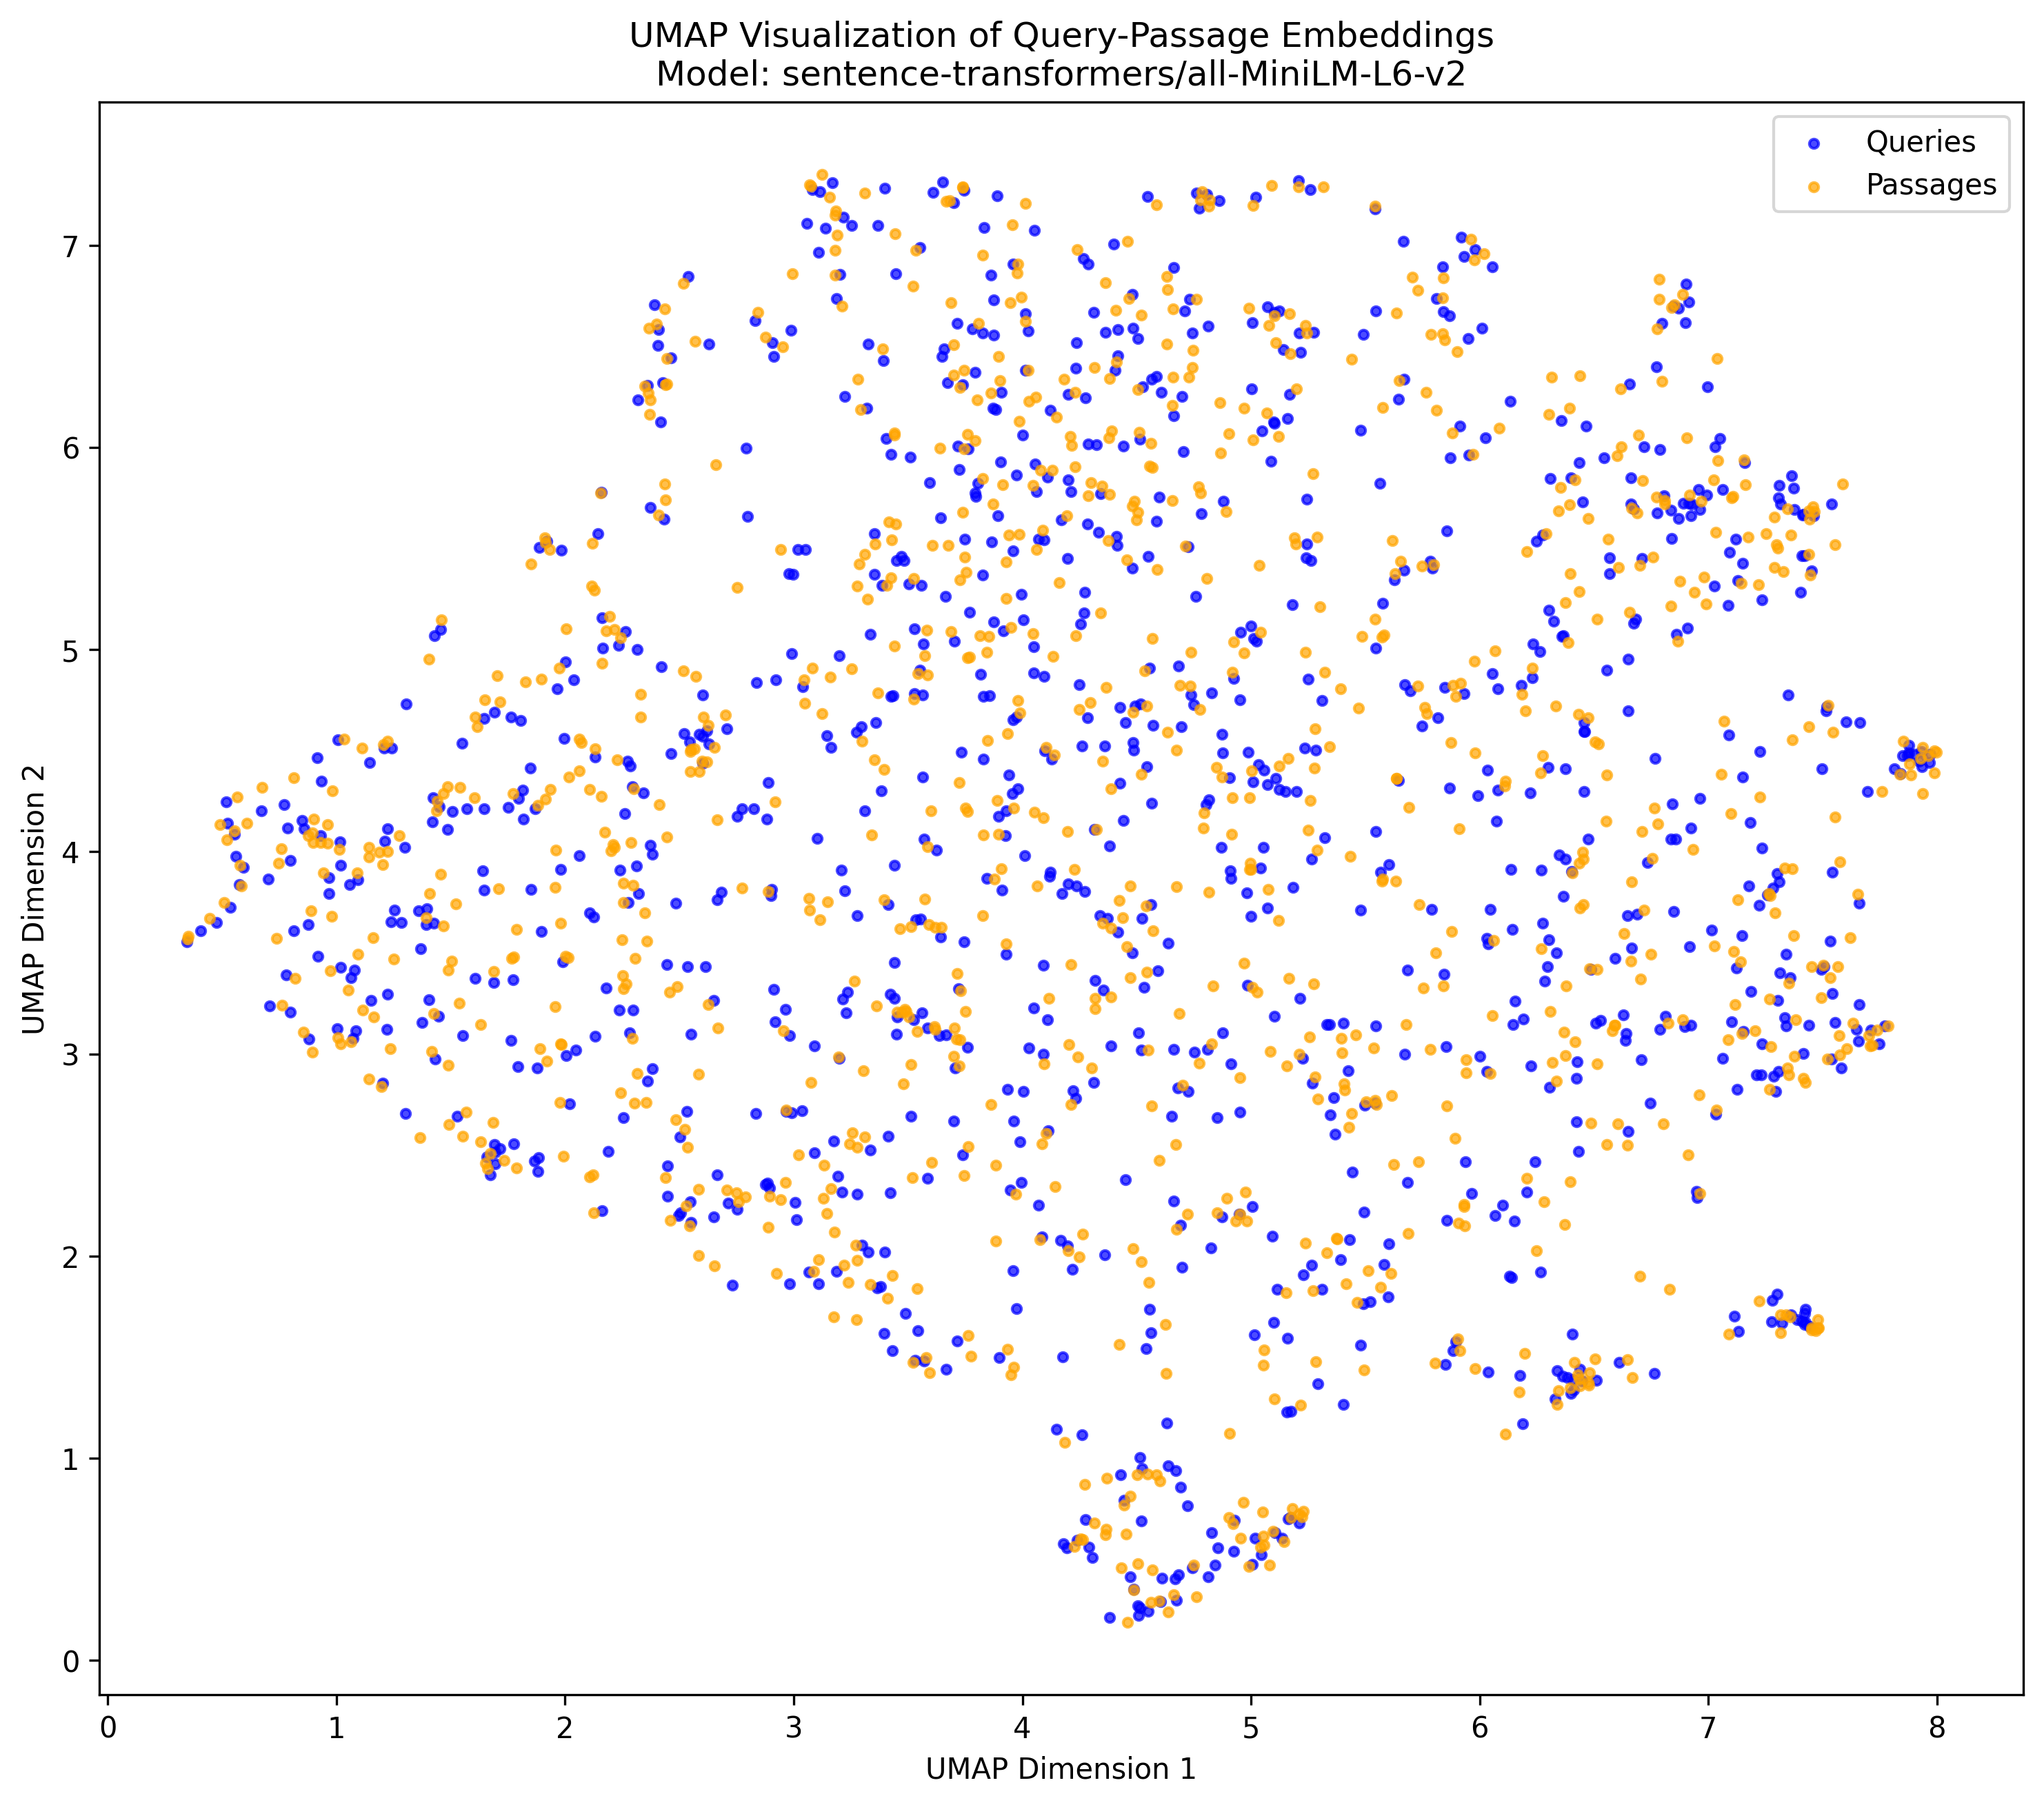
\includegraphics[width=\textwidth, height=0.75\textwidth, keepaspectratio]{umap_visualization_sentence_transformers_all_MiniLM_L6_v2.png}
\caption{Base SBERT: Well-defined semantic clustering with natural boundaries and balanced distribution}
\label{fig:umap_base_thesis}
\end{subfigure}
\hfill
\begin{subfigure}{0.48\textwidth}
\centering
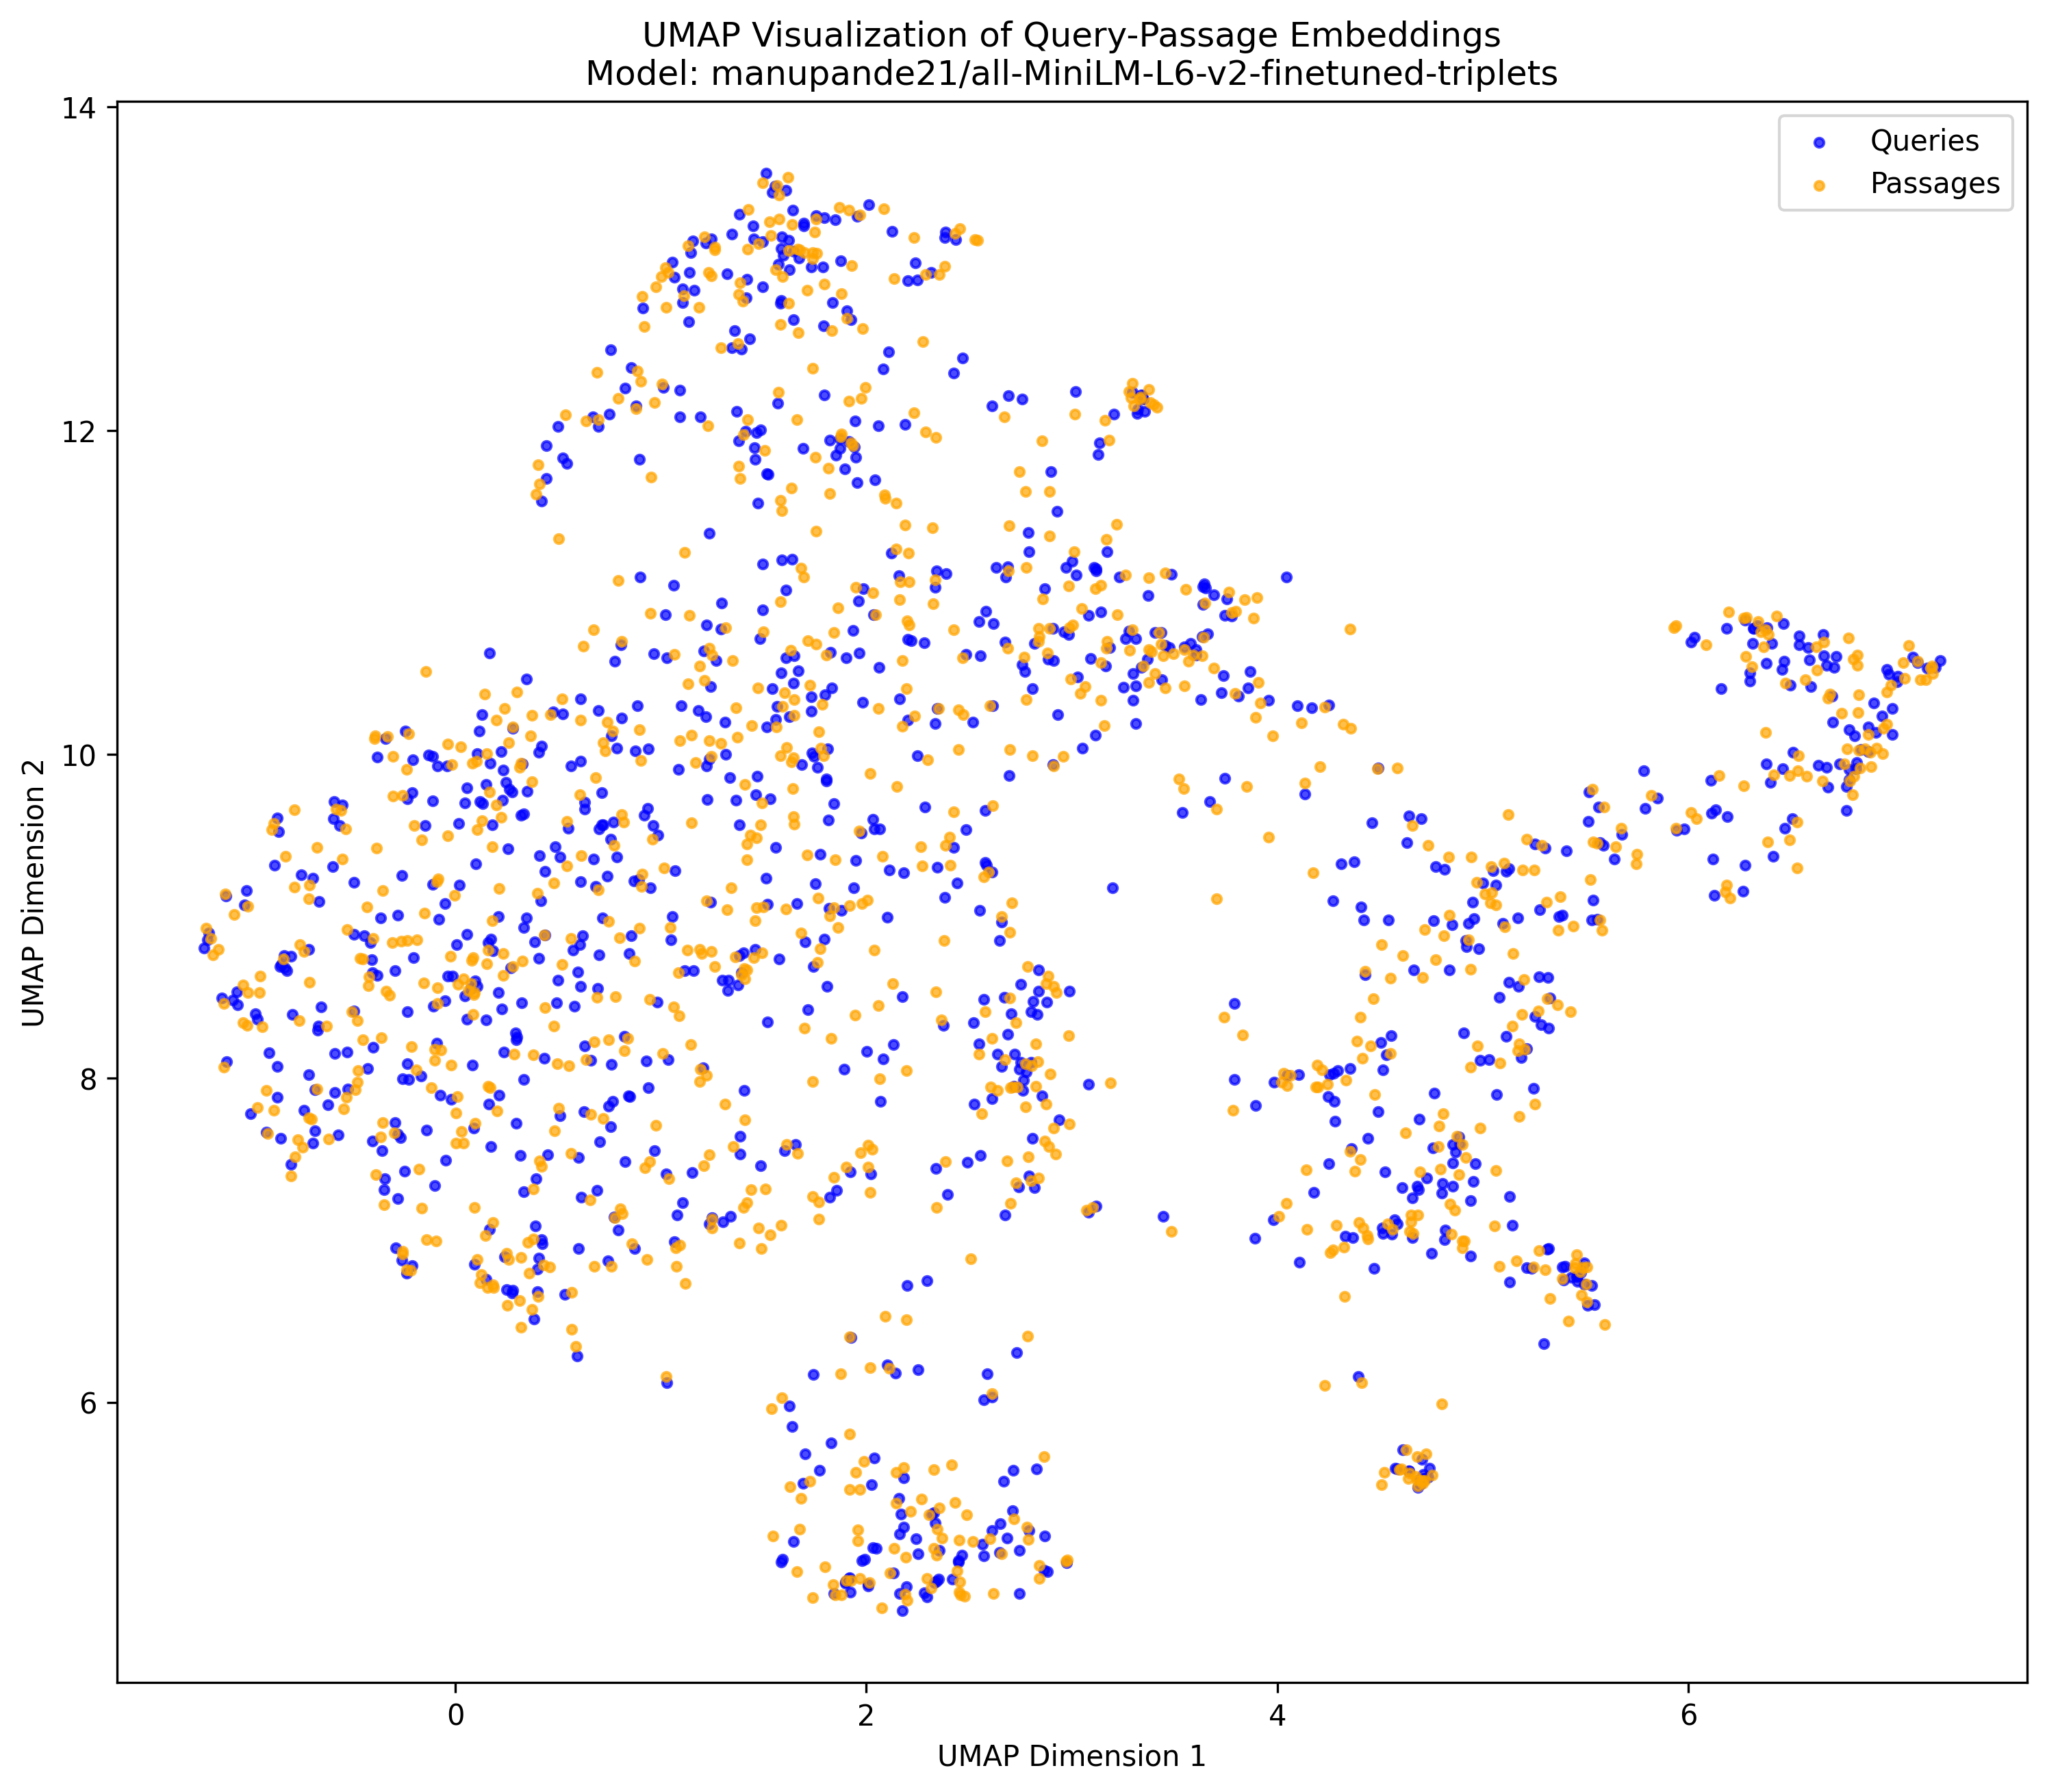
\includegraphics[width=\textwidth, height=0.75\textwidth, keepaspectratio]{umap_visualization_manupande21_all_MiniLM_L6_v2_finetuned_triplets.png}
\caption{Full FT (Random): Distinct island formations with preserved but altered clustering structure}
\label{fig:umap_full_random_thesis}
\end{subfigure}

\vspace{0.8cm}

% Second row: Full FT Hard and LoRA Random
\begin{subfigure}{0.48\textwidth}
\centering
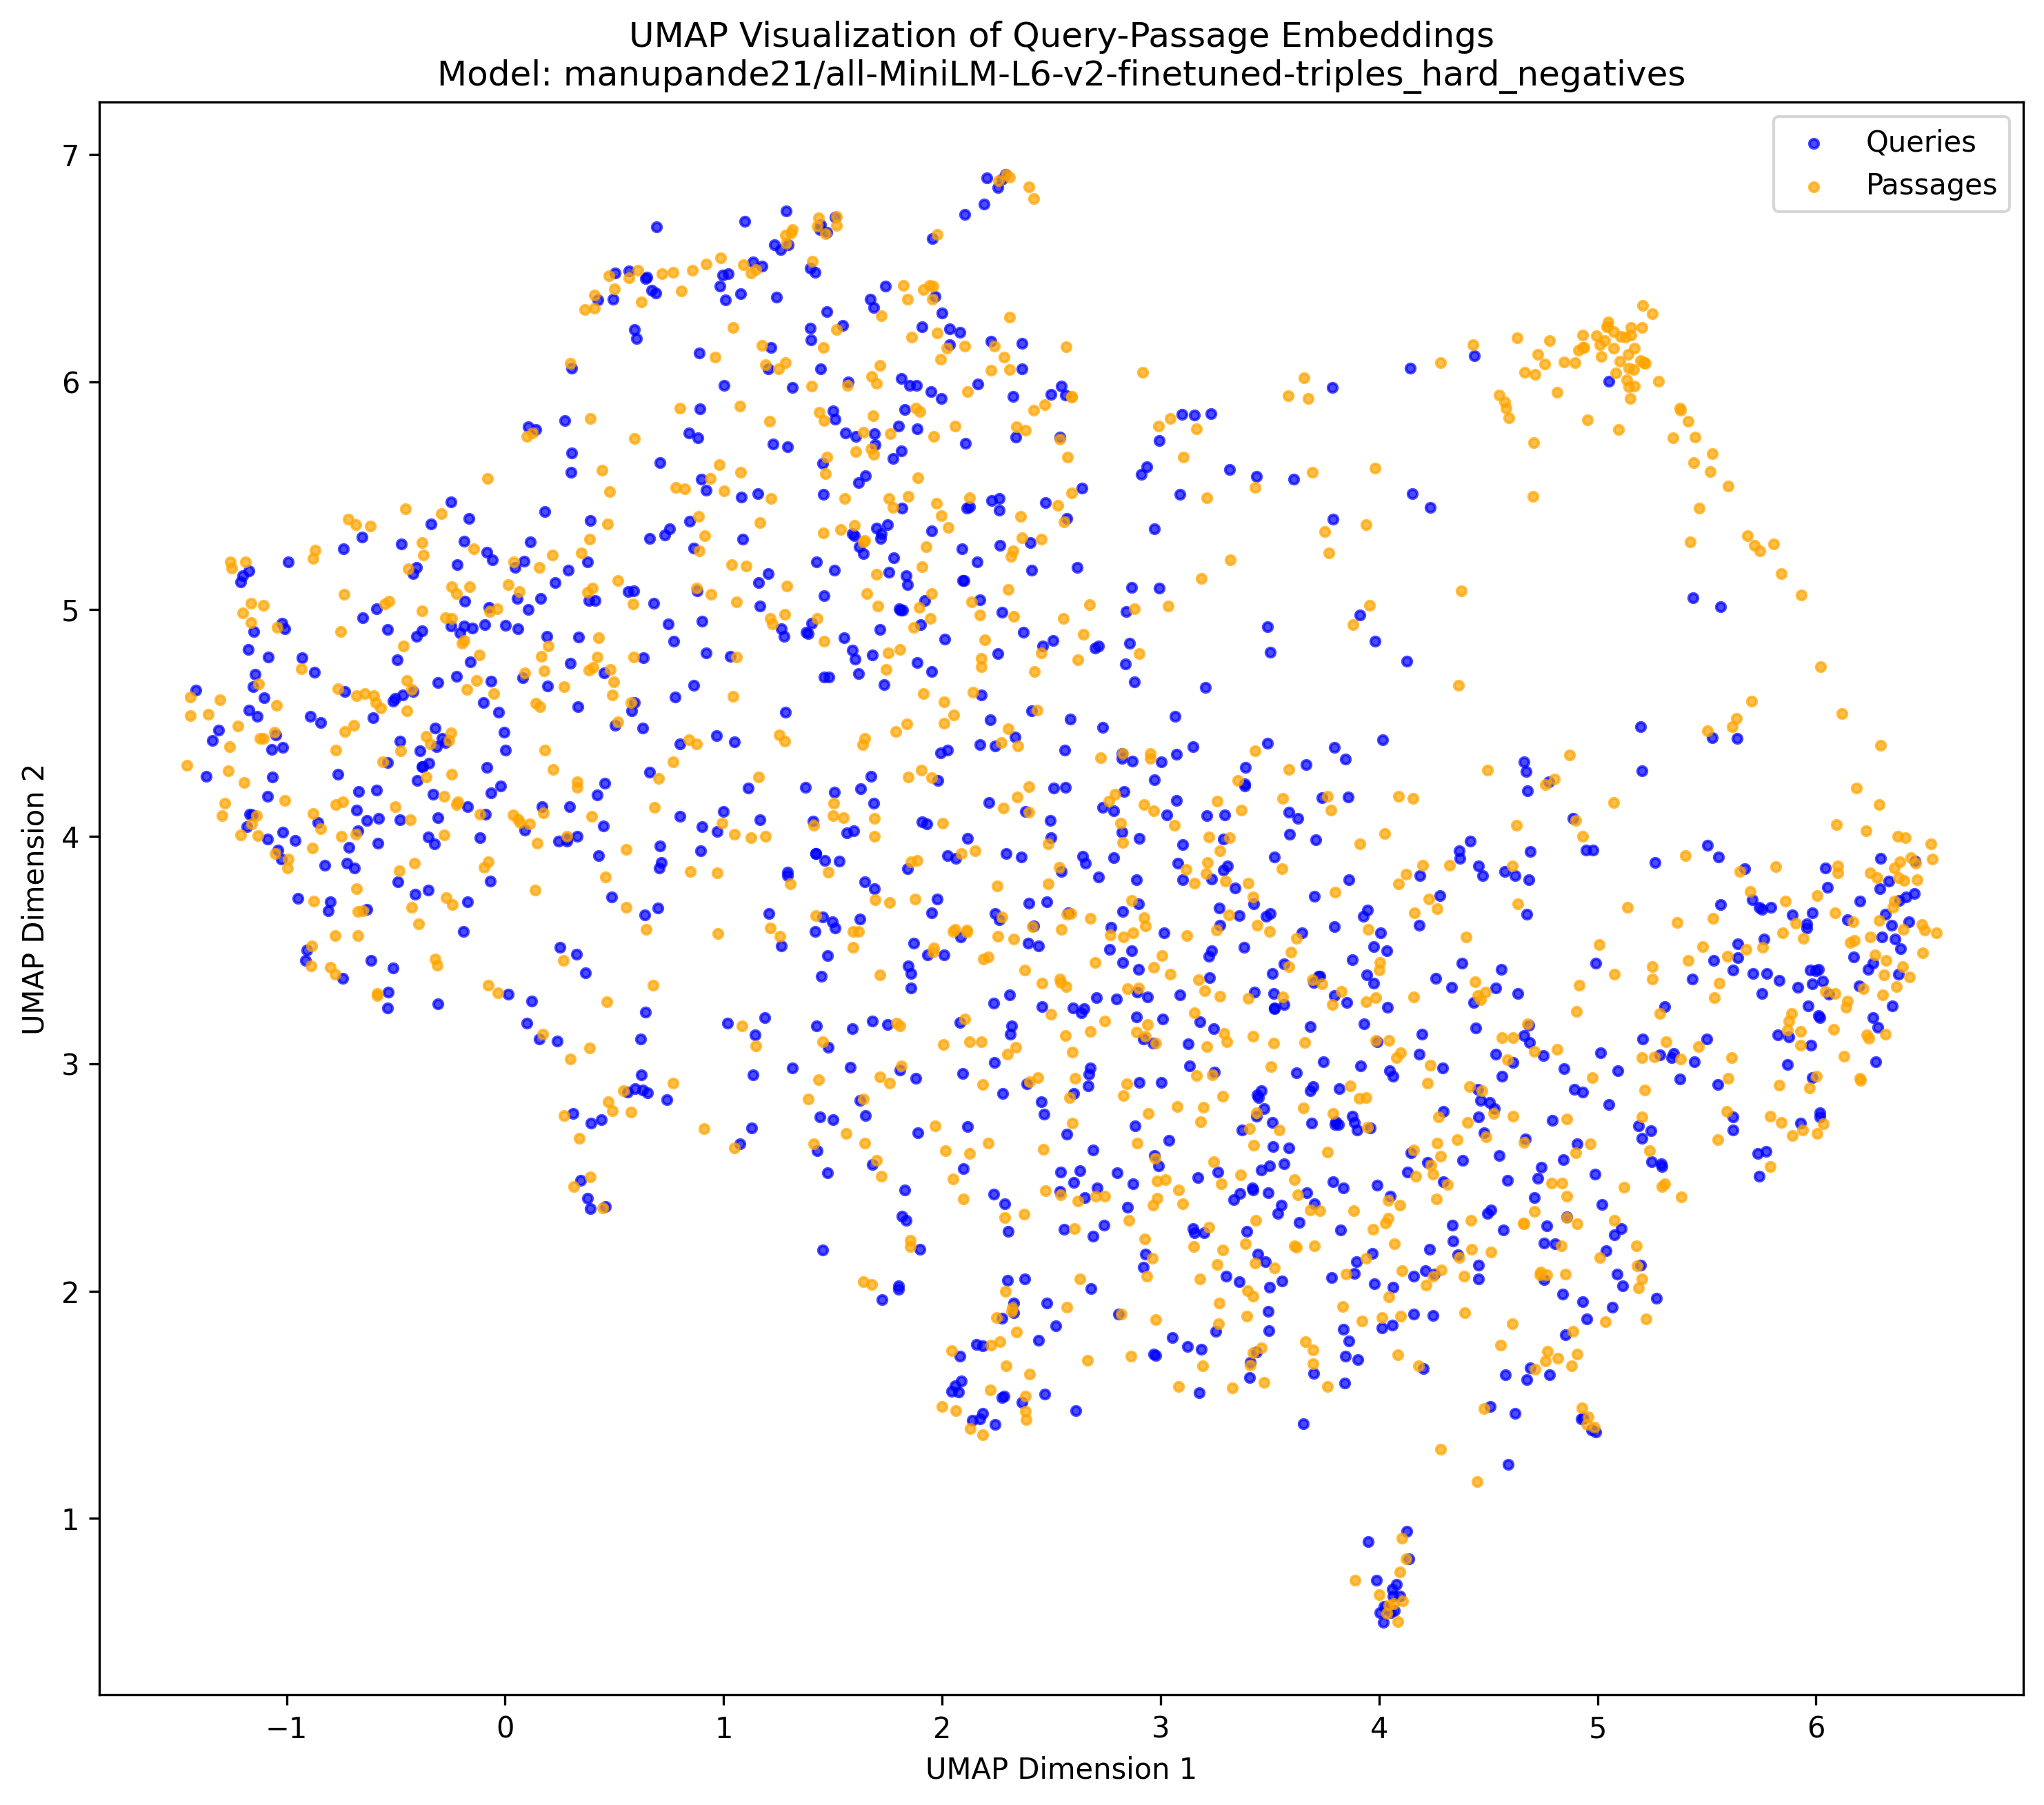
\includegraphics[width=\textwidth, height=0.75\textwidth, keepaspectratio]{umap_visualization_manupande21_all_MiniLM_L6_v2_finetuned_triples_hard_negatives.png}
\caption{Full FT (Hard): Increased uniformity showing moderate embedding space flattening}
\label{fig:umap_full_hard_thesis}
\end{subfigure}
\hfill
\begin{subfigure}{0.48\textwidth}
\centering
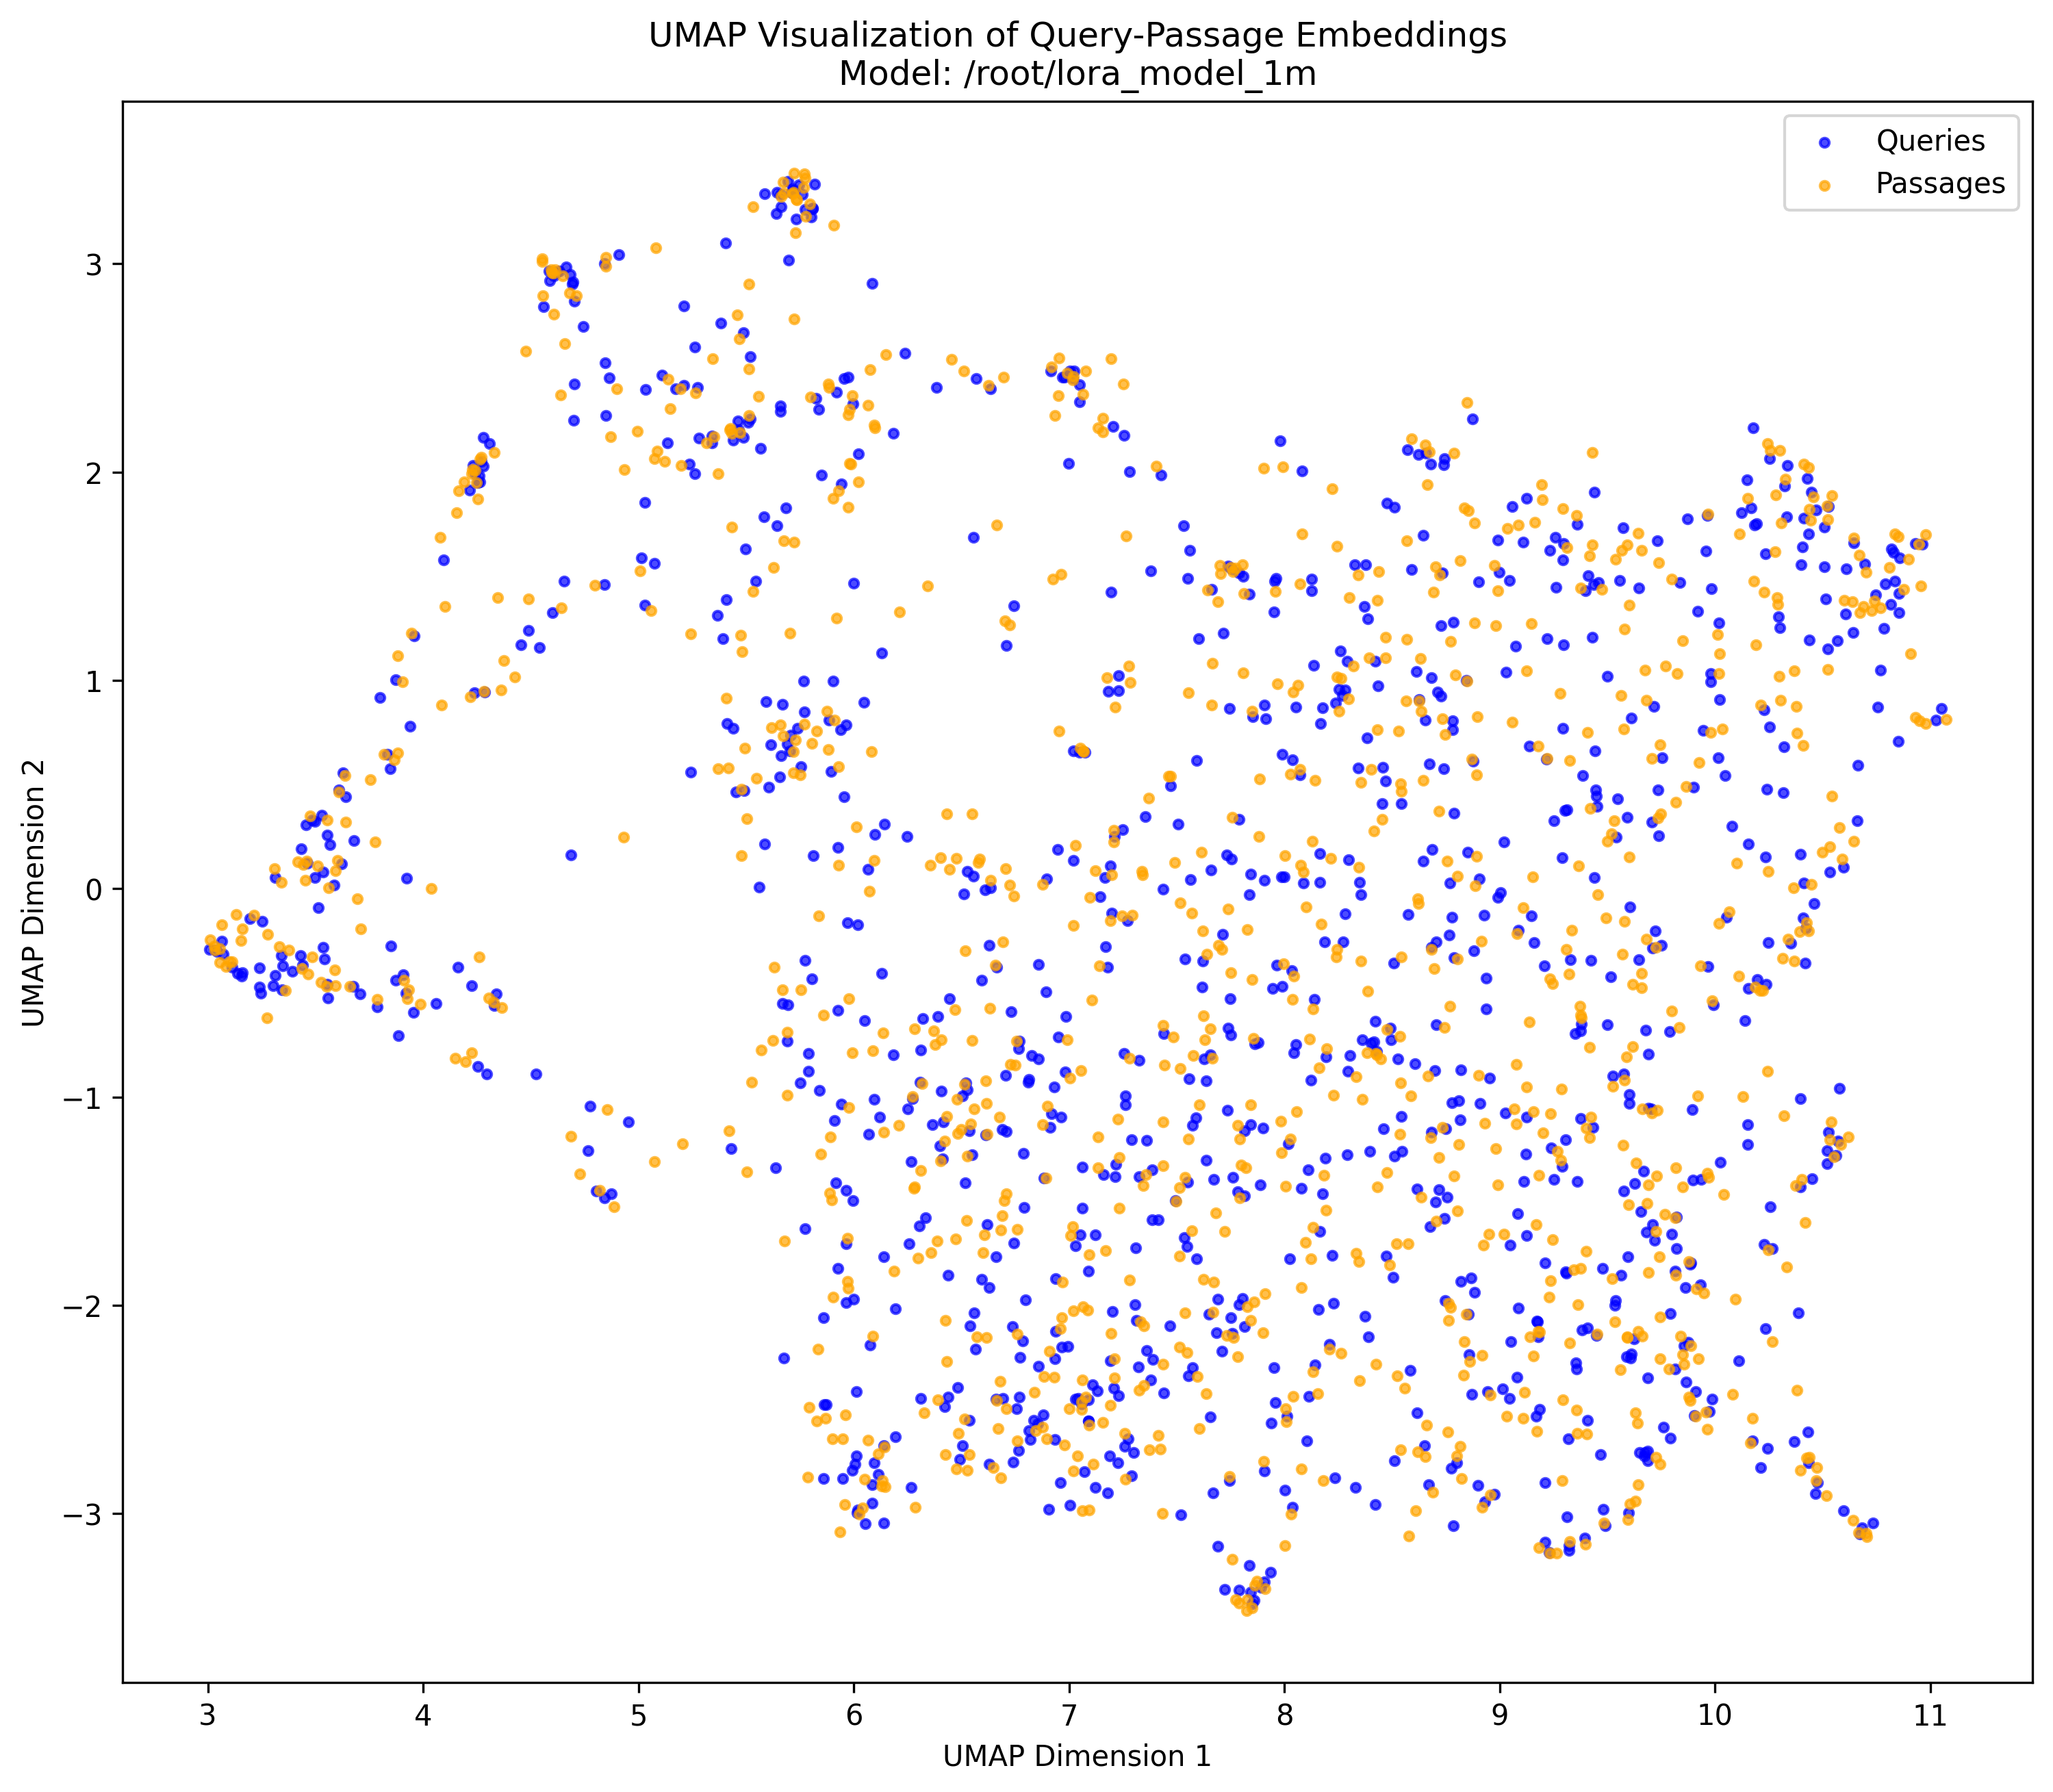
\includegraphics[width=\textwidth, height=0.75\textwidth, keepaspectratio]{umap_visualization__root_lora_model_1m.png}
\caption{LoRA FT (Random): Reduced semantic differentiation with compressed clustering}
\label{fig:umap_lora_random_thesis}
\end{subfigure}

\vspace{0.8cm}

% Third row: LoRA Hard (centered)
\begin{subfigure}{0.48\textwidth}
\centering
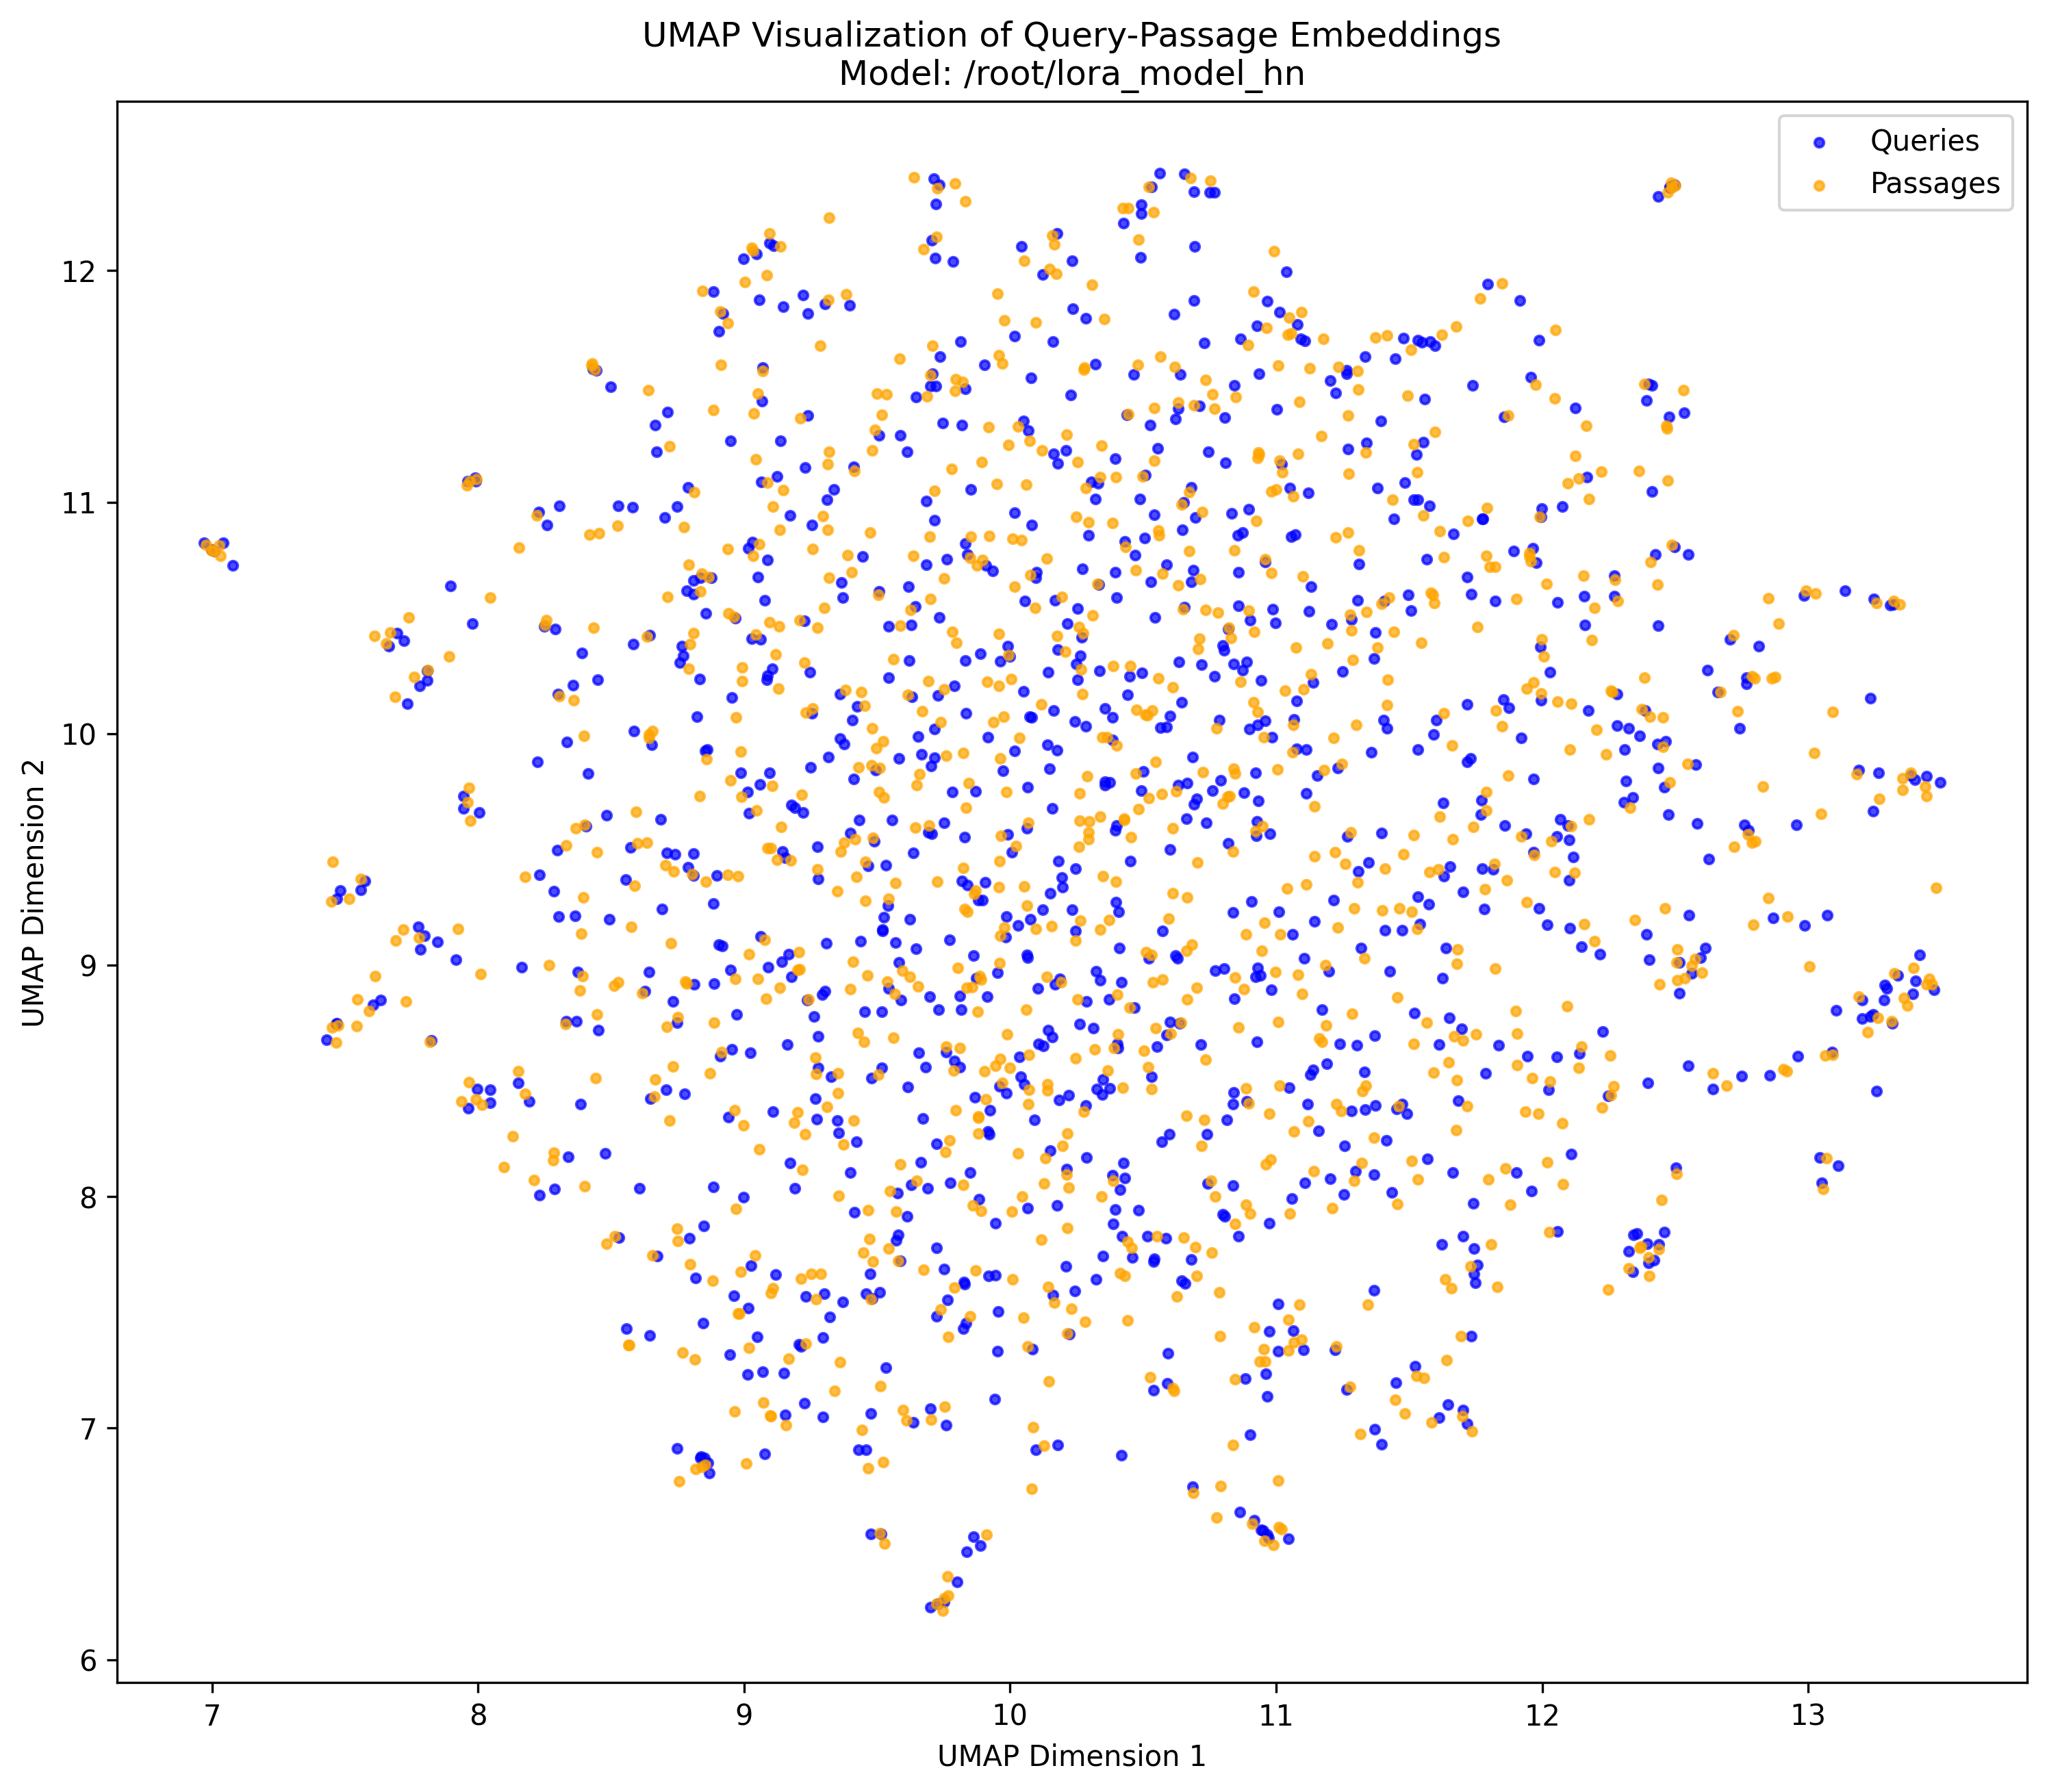
\includegraphics[width=\textwidth, height=0.75\textwidth, keepaspectratio]{umap_visualization__root_lora_model_hn.png}
\caption{LoRA FT (Hard): Maximum uniformity demonstrating catastrophic embedding space collapse}
\label{fig:umap_lora_hard_thesis}
\end{subfigure}

\caption{UMAP visualization of embedding spaces. Blue points represent query embeddings and orange points represent positive passage embeddings from 1,000 randomly sampled query-passage pairs. The progression demonstrates increasing embedding space uniformity.}
\label{fig:umap_all_thesis}
\end{figure*}

\subsection{Embedding Space Degradation Analysis}

The visualization reveals a clear degradation progression:

\begin{enumerate}
\item \textbf{Base Model (Figure~\ref{fig:umap_base_thesis}):} Well-structured semantic organization with distinct clusters and clear boundaries between different semantic regions
\item \textbf{Full FT Random (Figure~\ref{fig:umap_full_random_thesis}):} Island formations indicating preserved clustering but altered geometric relationships
\item \textbf{Full FT Hard (Figure~\ref{fig:umap_full_hard_thesis}):} Increased uniformity showing moderate flattening of the embedding space
\item \textbf{LoRA Random (Figure~\ref{fig:umap_lora_random_thesis}):} Reduced semantic differentiation with compressed clustering patterns
\item \textbf{LoRA Hard (Figure~\ref{fig:umap_lora_hard_thesis}):} Complete uniformity demonstrating catastrophic embedding space collapse
\end{enumerate}

\section{Training Dynamics Analysis}

\subsection{Loss Convergence Patterns}

Figure~\ref{fig:training_curves_thesis} illustrates the training loss trajectories for all four fine-tuned models, providing insights into convergence behavior and optimization challenges.

\begin{figure*}[t]
\centering
\begin{subfigure}{0.48\textwidth}
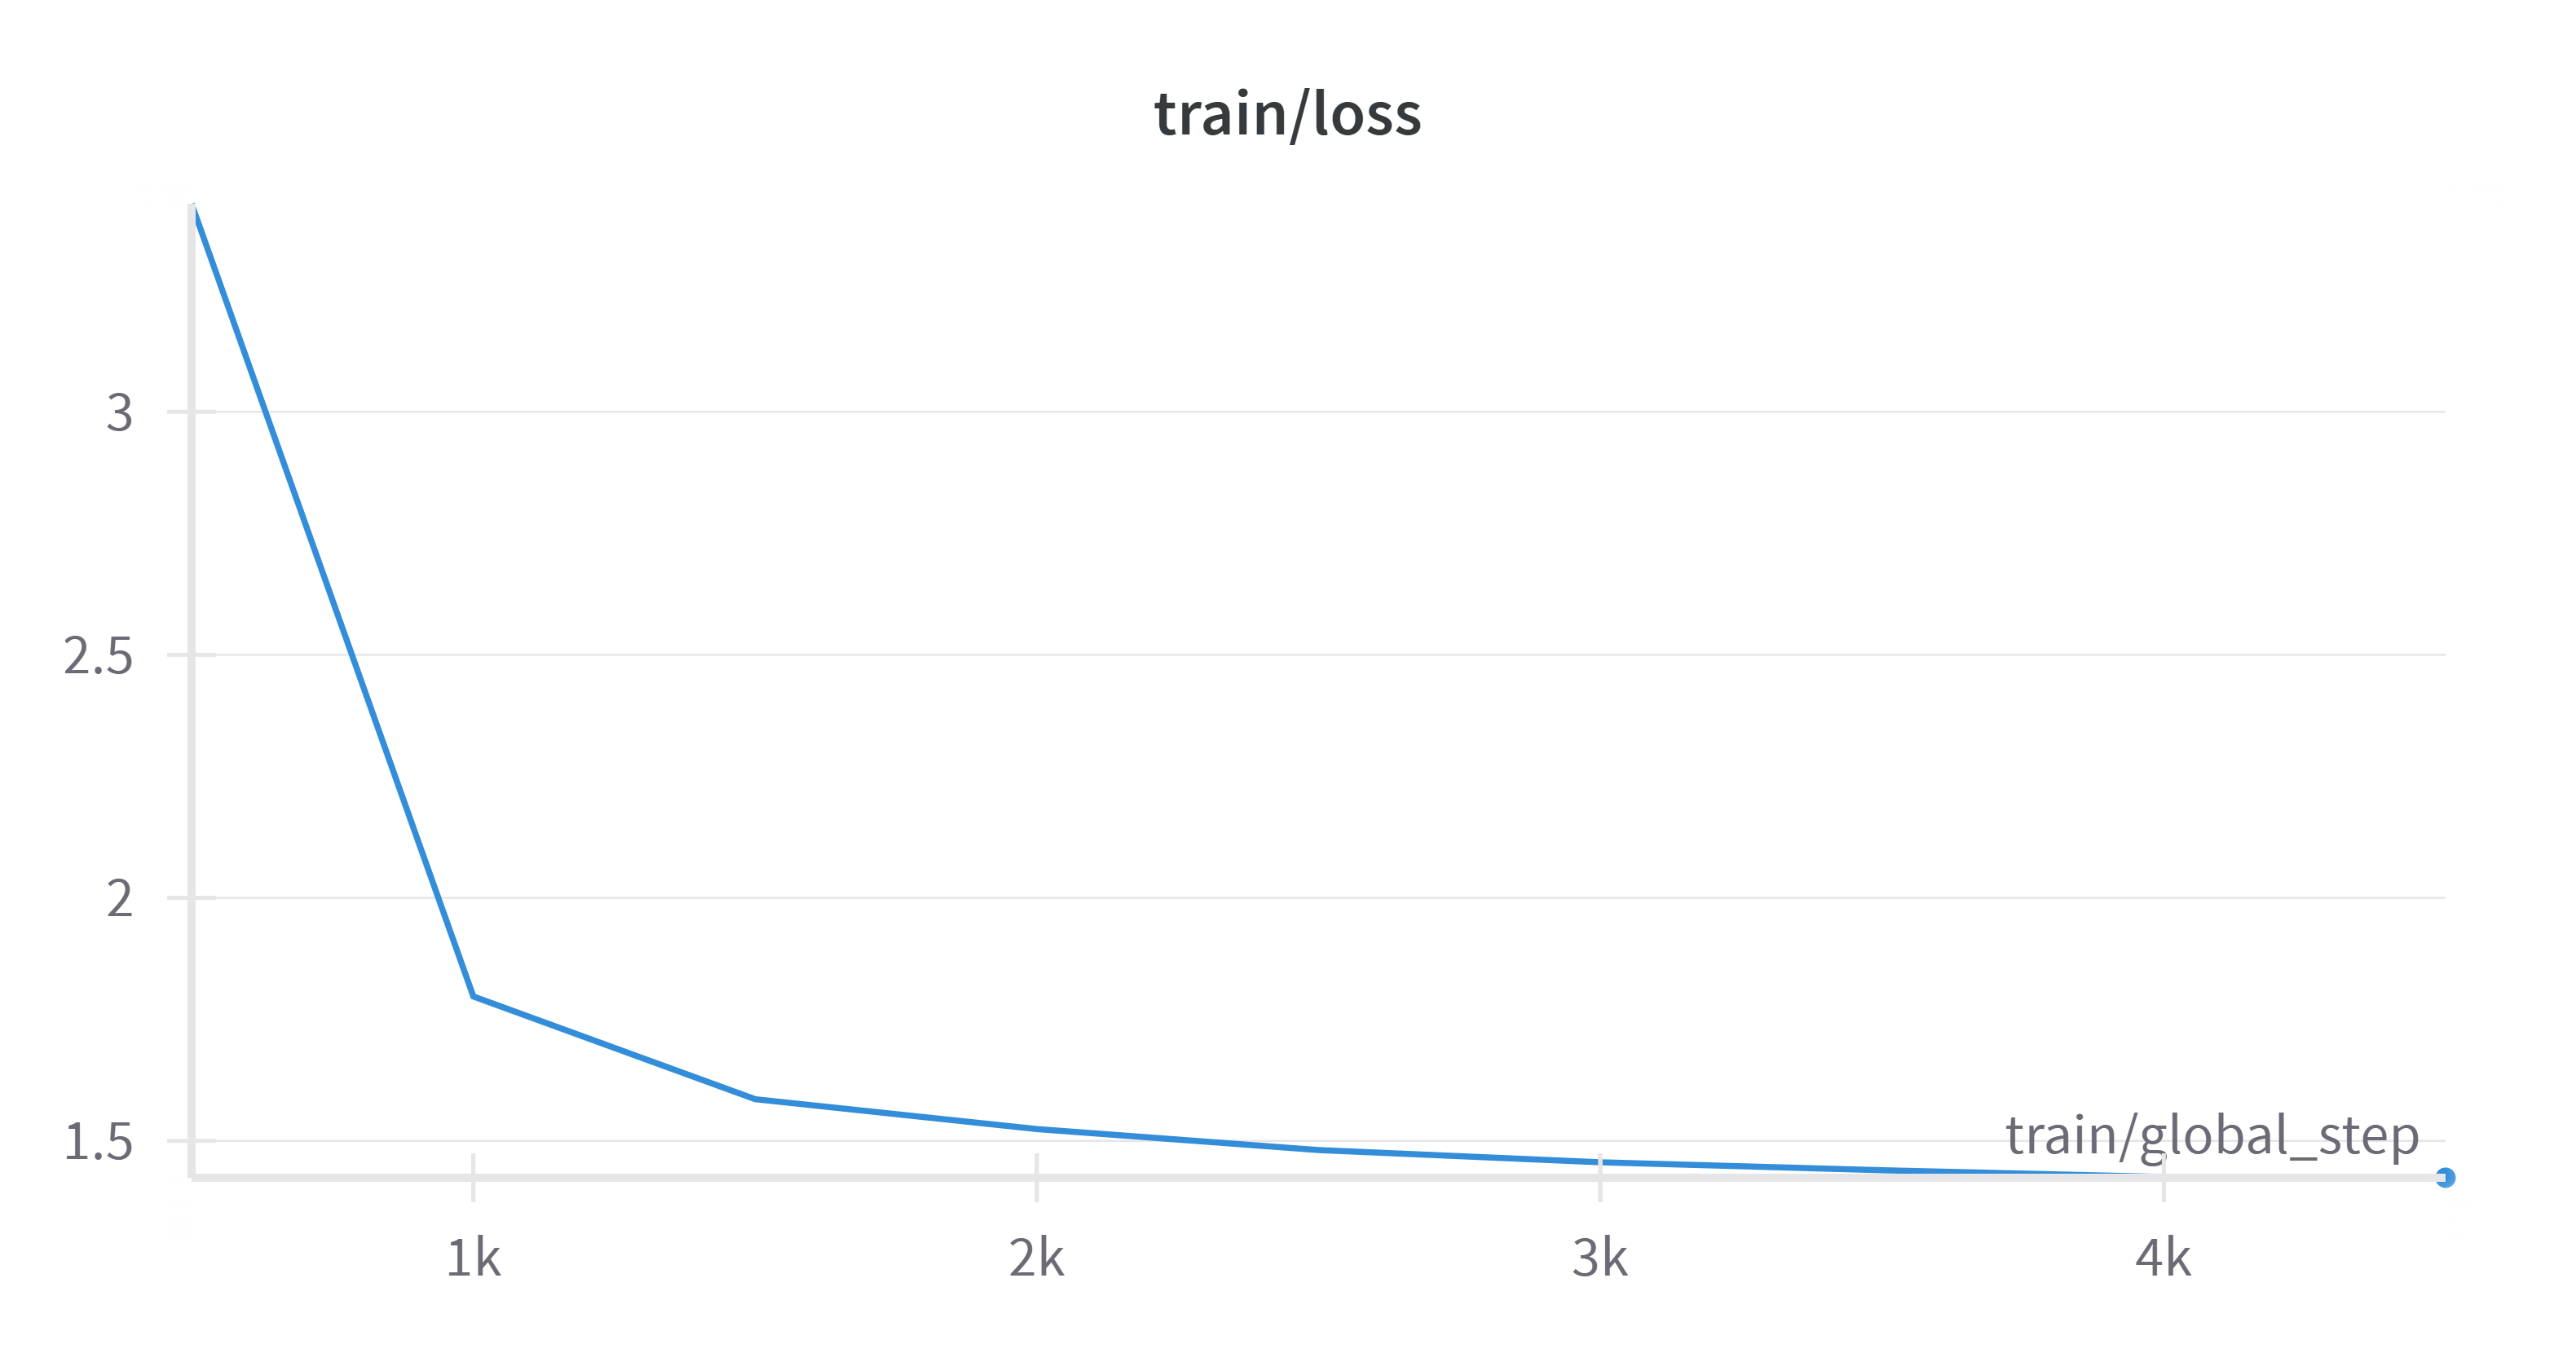
\includegraphics[width=\textwidth]{lora_finetuned_1million.png}
\caption{LoRA FT (Random): Steady convergence but higher final loss compared to full fine-tuning}
\end{subfigure}
\hfill
\begin{subfigure}{0.48\textwidth}
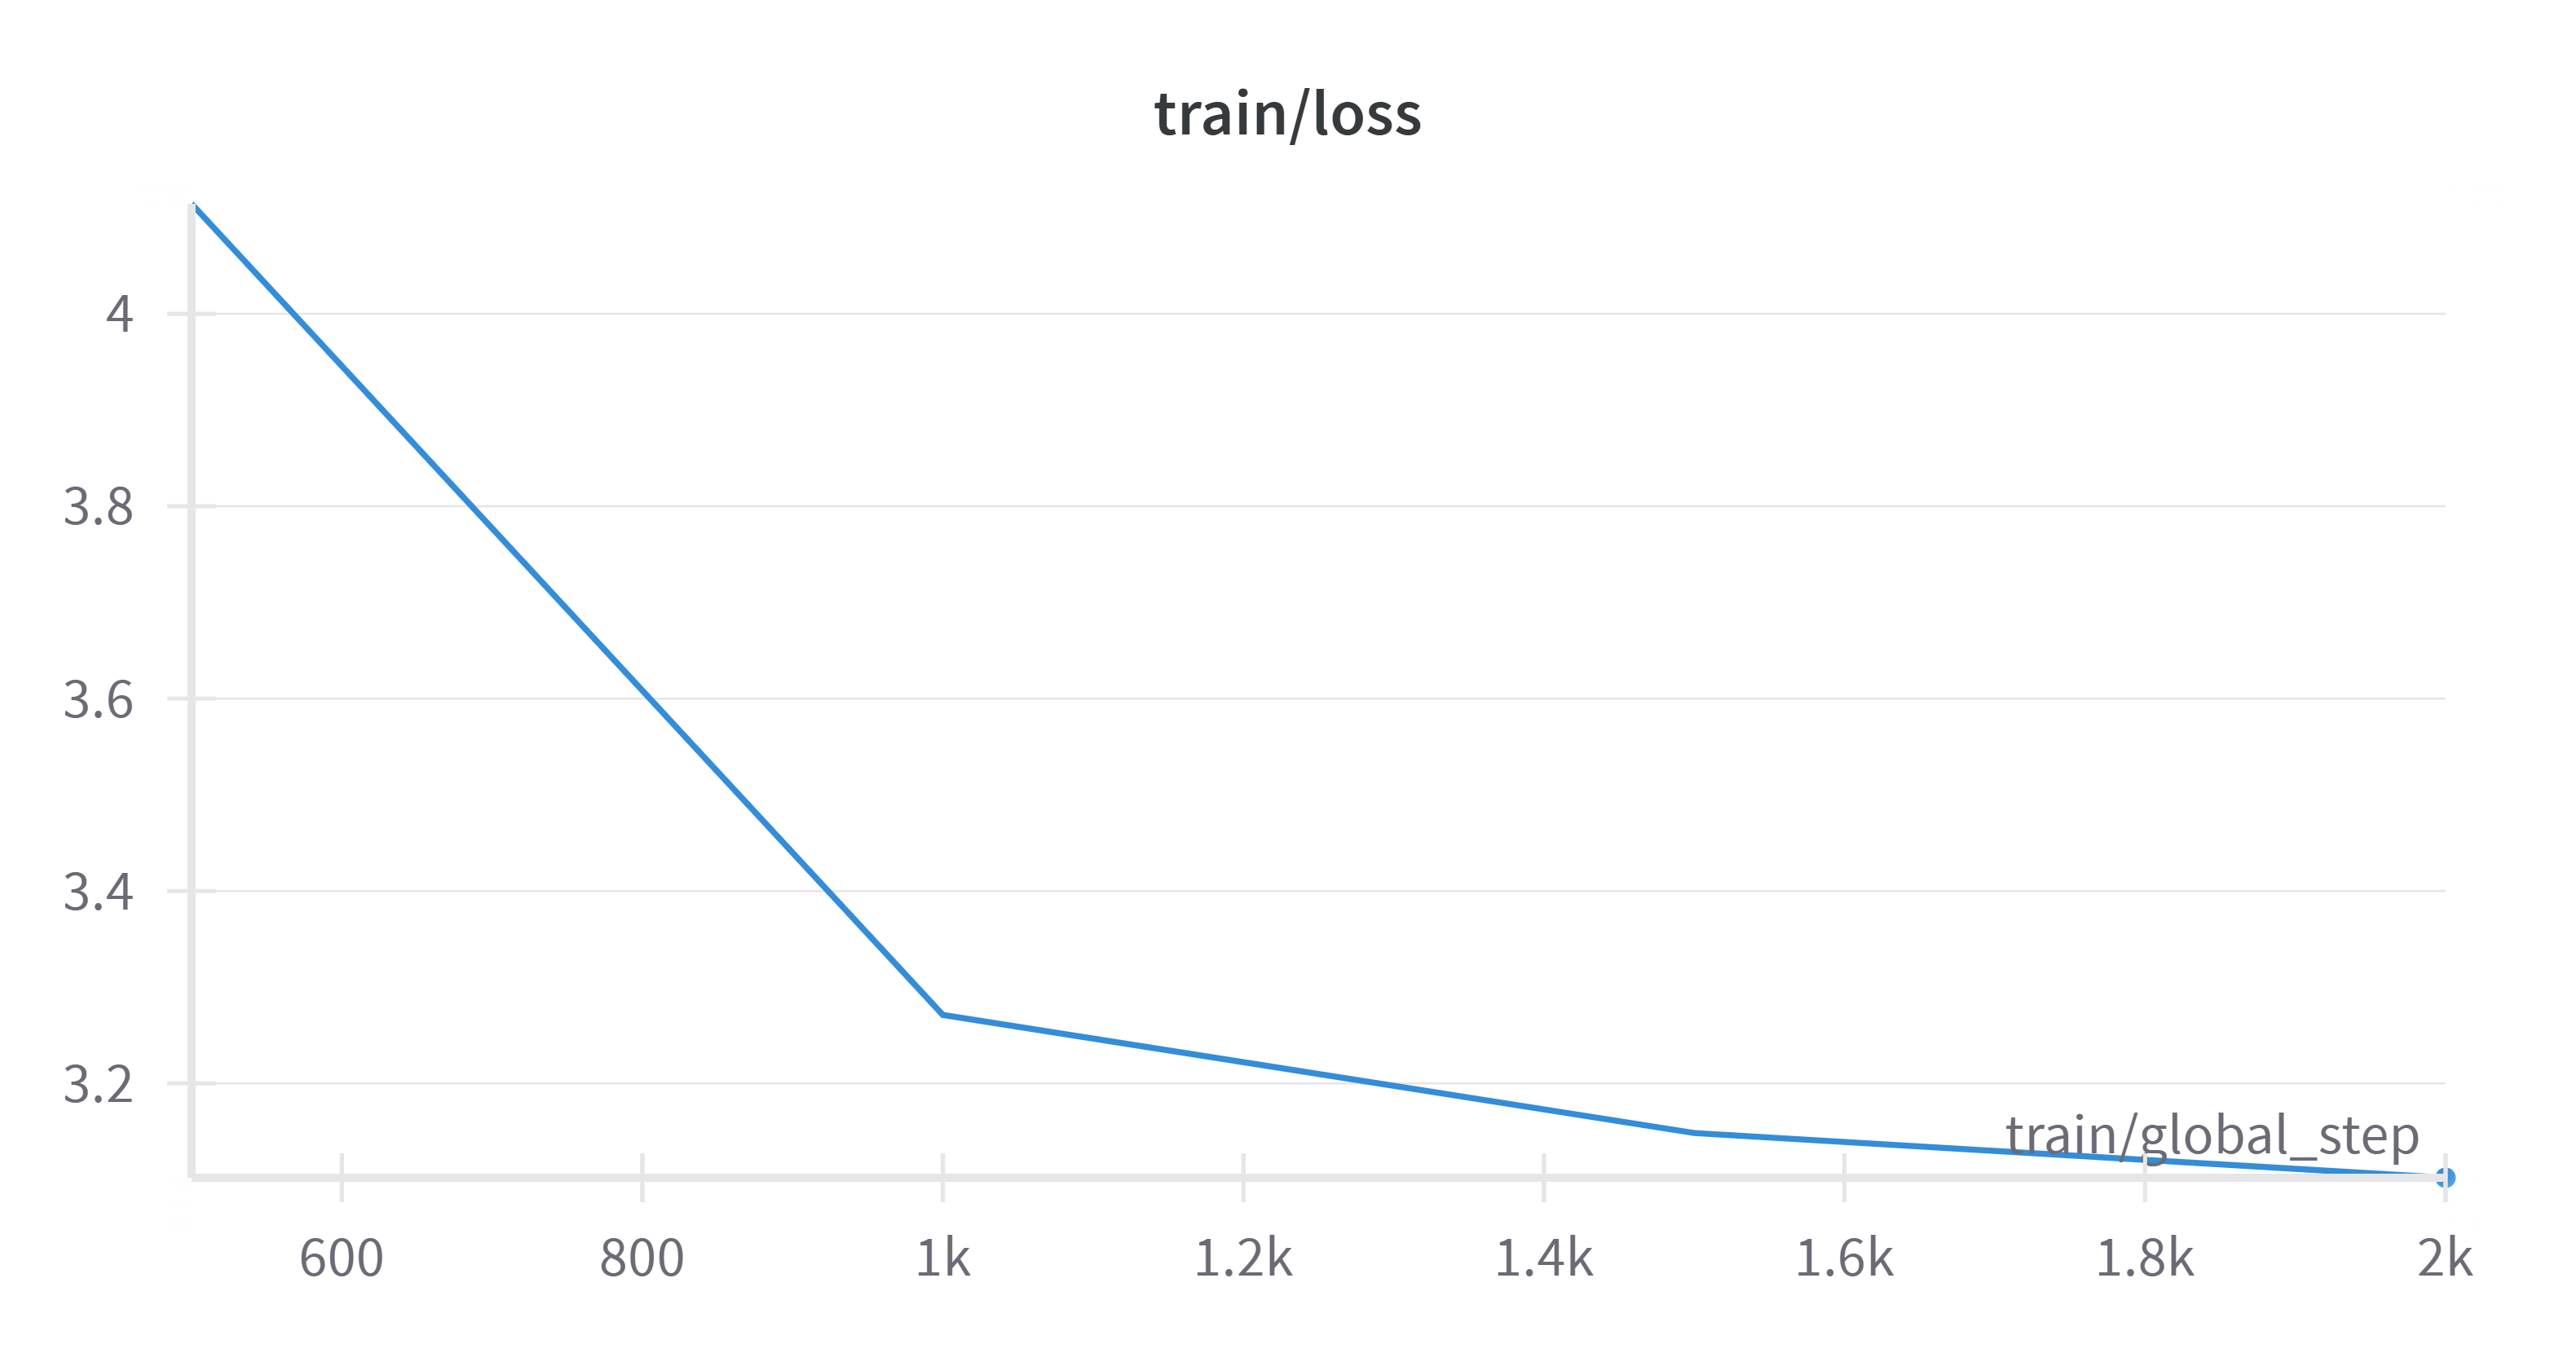
\includegraphics[width=\textwidth]{lora_finetuned_hard_negatives.png}
\caption{LoRA FT (Hard): Training instability and poor convergence leading to highest final loss}
\end{subfigure}

\begin{subfigure}{0.48\textwidth}
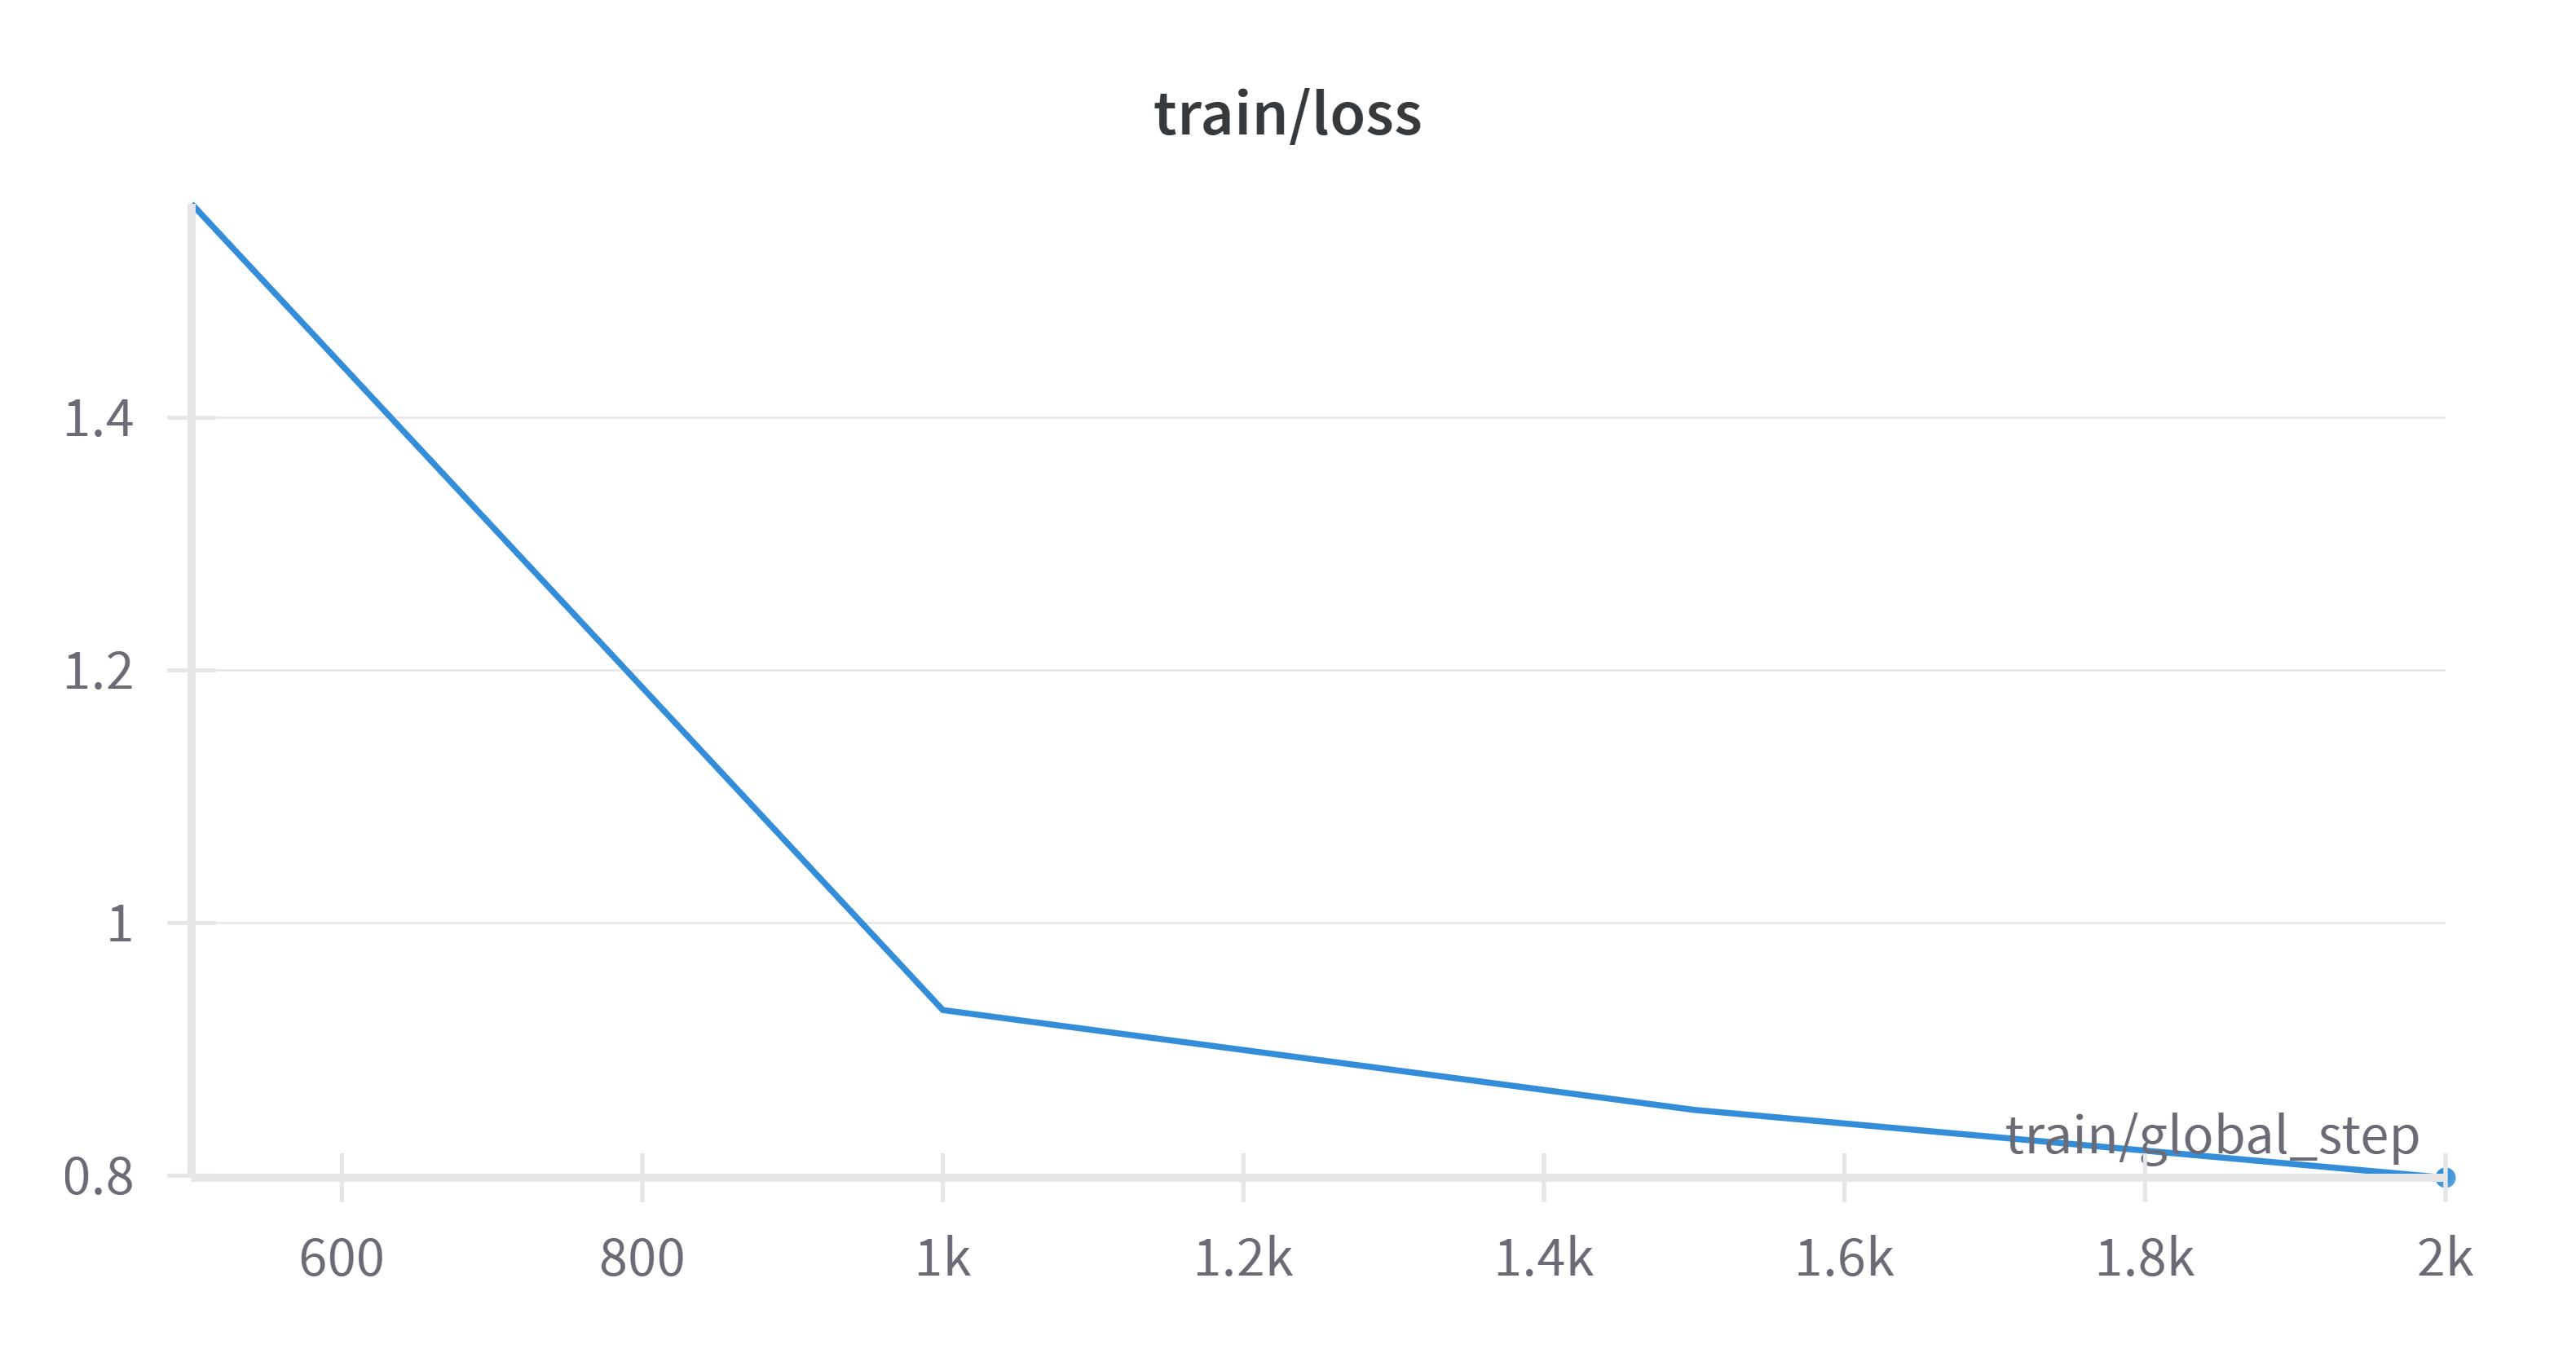
\includegraphics[width=\textwidth]{sbert_finetuned_1million.png}
\caption{Full FT (Random): Smooth optimization achieving lowest training loss across all variants}
\end{subfigure}
\hfill
\begin{subfigure}{0.48\textwidth}
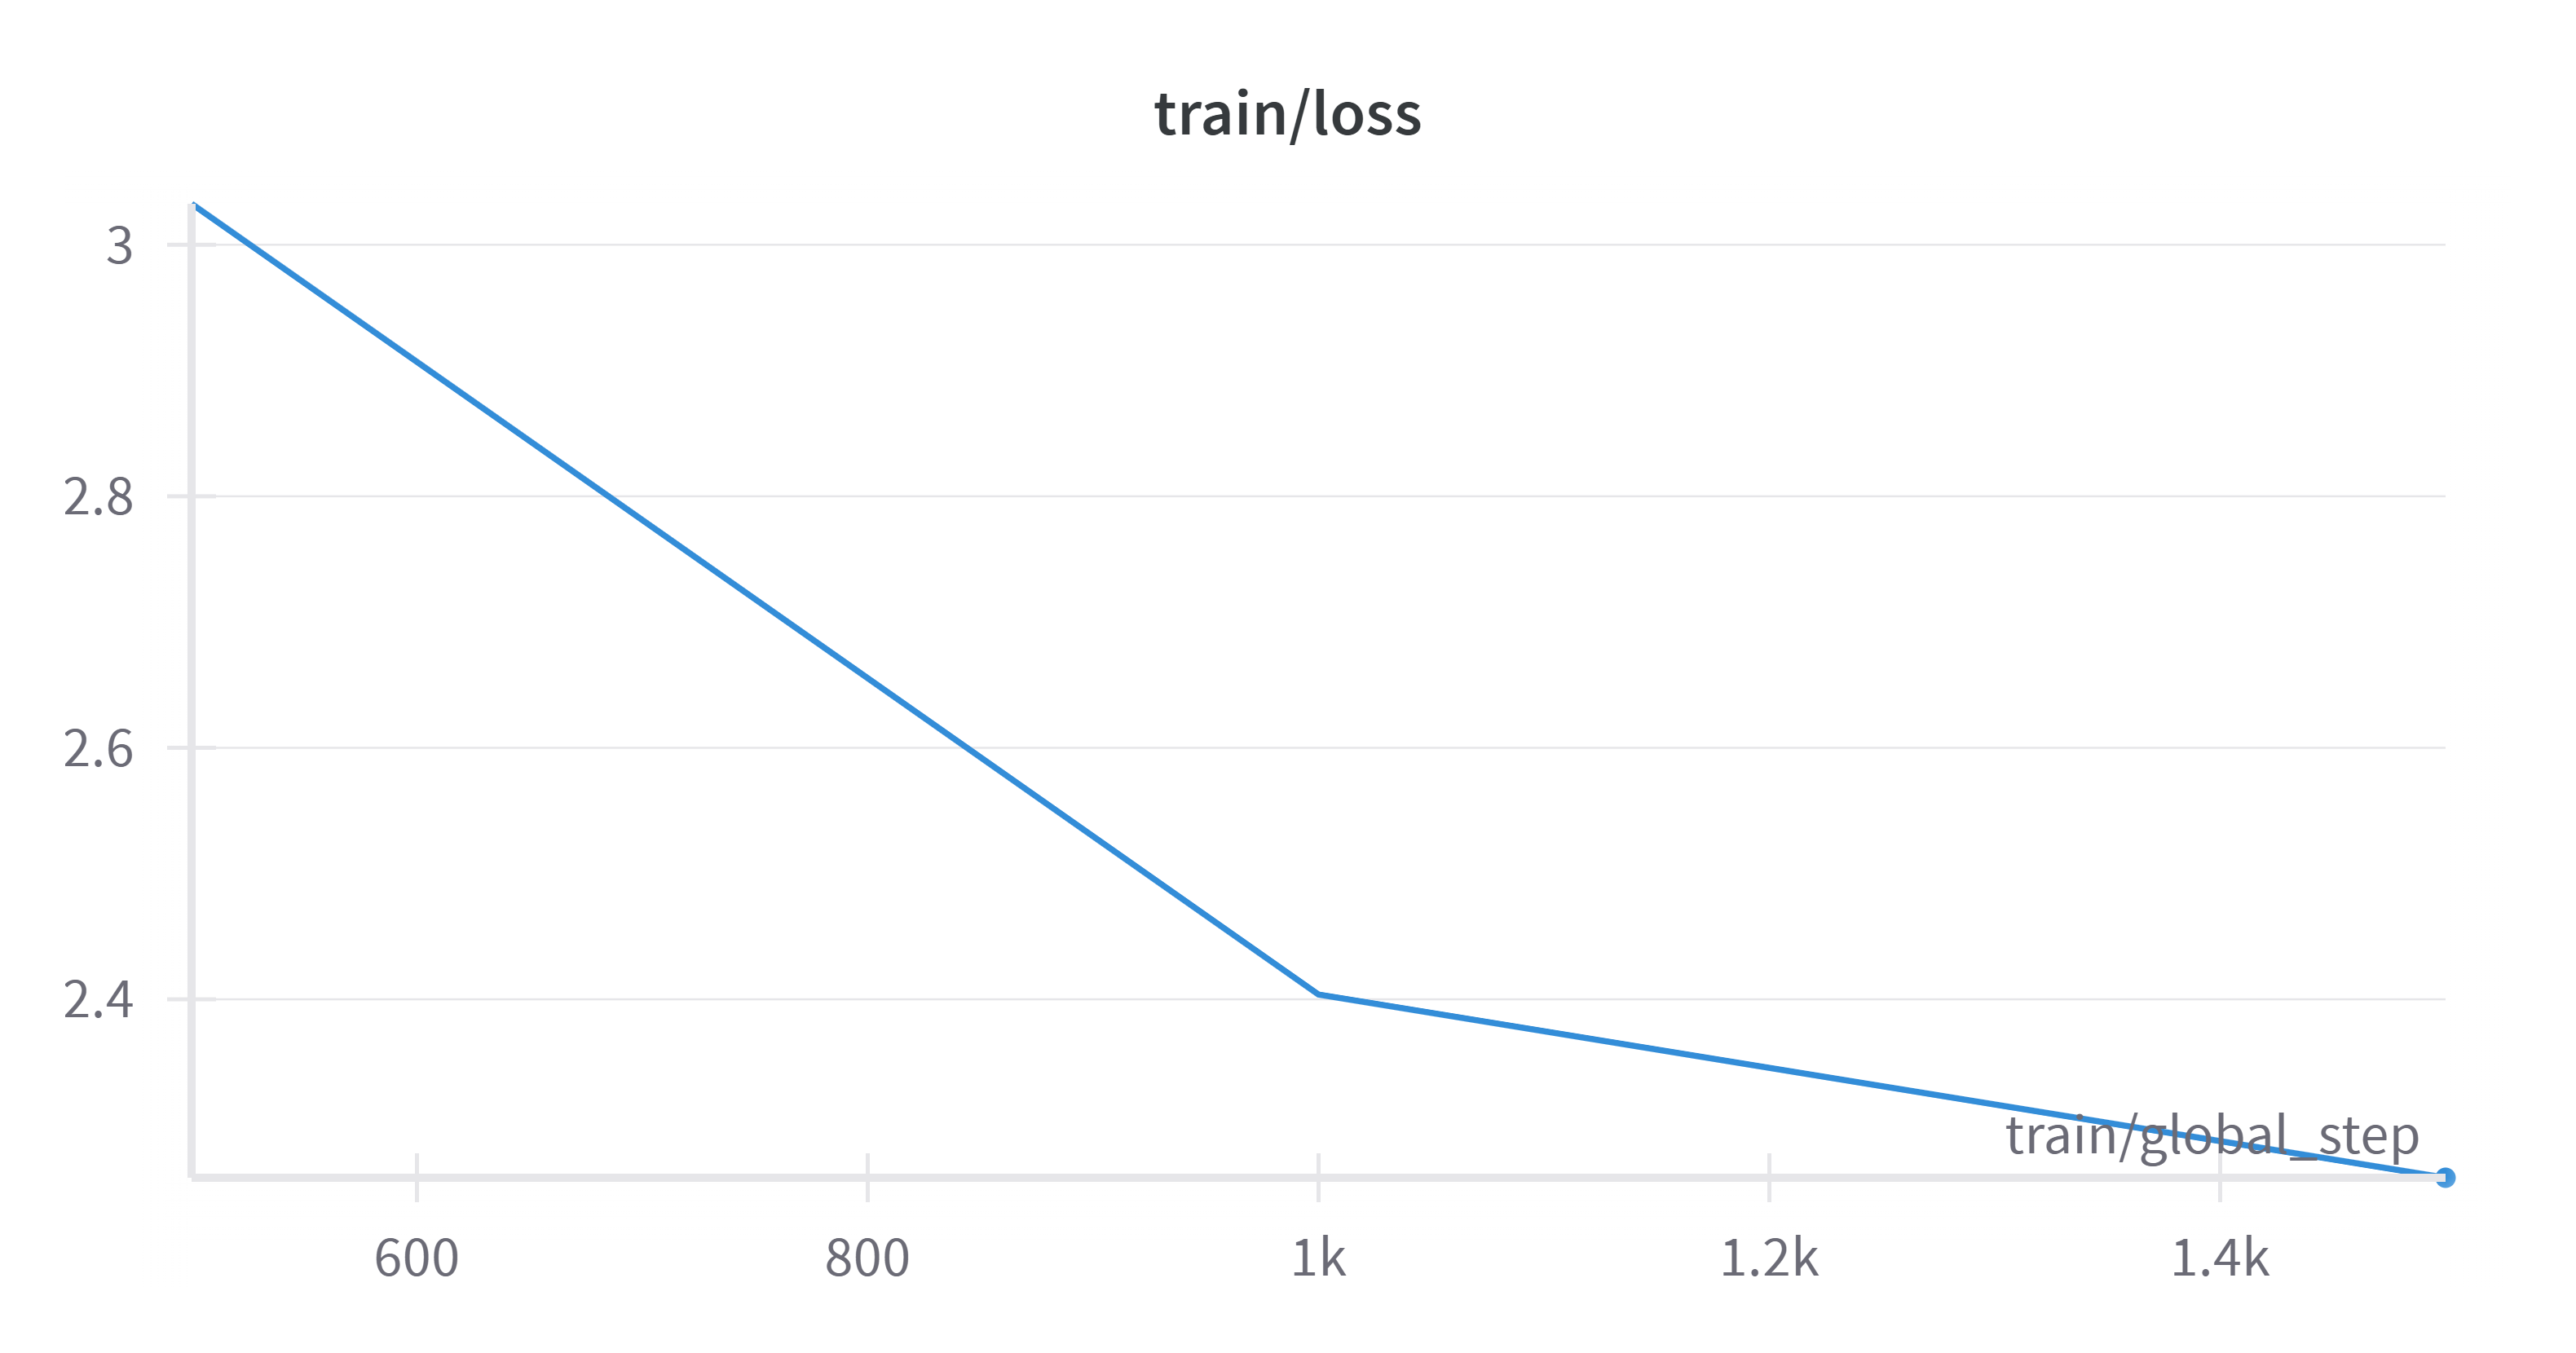
\includegraphics[width=\textwidth]{sbert_finetuned_hard_negatives.png}
\caption{Full FT (Hard): Rapid initial loss reduction followed by convergence challenges}
\end{subfigure}
\caption{Training loss curves revealing convergence patterns across different fine-tuning approaches and negative sampling strategies.}
\label{fig:training_curves_thesis}
\end{figure*}

\subsection{Training Convergence Metrics}

Table~\ref{tab:training_metrics_thesis} presents quantitative training convergence metrics including final training loss and cosine similarity accuracy.

\begin{table}[h]
\centering
\caption{Training Convergence Metrics}
\label{tab:training_metrics_thesis}
\begin{tabular}{lcc}
\toprule
Model & Final Train Loss & Eval Cosine Accuracy \\
\midrule
Full FT (Random) & 0.79 & 0.97 \\
LoRA FT (Random) & 1.42 & 0.95 \\
Full FT (Hard) & 2.26 & 0.84 \\
LoRA FT (Hard) & 3.10 & 0.78 \\
\bottomrule
\end{tabular}
\end{table}

\subsection{Training Dynamics Insights}

Combined analysis of training dynamics, loss curves, and convergence metrics reveals the true nature of fine-tuning failure:

\begin{itemize}
\item \textbf{Optimization Success vs. Performance:} Better training convergence among fine-tuned models correlates with better downstream performance, but all variants consistently underperform the base model
\item \textbf{Hard Negatives Impact:} Hard negatives cause training instability and higher final losses across both fine-tuning approaches
\item \textbf{LoRA Sensitivity:} LoRA shows greater sensitivity to negative sampling strategy, with particularly poor performance on hard negatives
\end{itemize}

\section{Comparative Analysis and Discussion}

\subsection{Cross-Method Performance Comparison}

When comparing across fine-tuning methods:

\begin{itemize}
\item \textbf{Full fine-tuning} consistently outperforms LoRA across both negative sampling strategies
\item \textbf{Random negatives} uniformly outperform hard negatives across both fine-tuning approaches
\item \textbf{Performance degradation severity} follows the pattern: LoRA Hard (-32.3\%) > Full Hard (-16.2\%) > LoRA Random (-15.5\%) > Full Random (-13.5\%)
\end{itemize}

\subsection{The Scale Disparity Effect}

The consistent underperformance across all variants strongly suggests that the fundamental issue lies in scale disparity rather than methodological choices. The base model's exposure to 9.1M MS MARCO samples during billion-scale pre-training creates an optimization landscape that cannot be meaningfully improved through 1M-sample fine-tuning.

\subsection{Embedding Space as Diagnostic Tool}

The strong correlation between embedding space degradation (visualized through UMAP) and performance degradation (measured through MRR) validates our diagnostic methodology. This correlation suggests that embedding space analysis should become standard practice in fine-tuning research, particularly when working with pre-optimized models.

\section{Validation of Hypotheses}

\subsection{H1: Universal Fine-Tuning Degradation - CONFIRMED}

All fine-tuning approaches underperformed the base model with statistical significance, confirming our hypothesis about saturated benchmark effects.

\subsection{H2: Hard Negatives Paradox - CONFIRMED}

Hard negatives consistently harmed performance more than random negatives across both fine-tuning approaches, confirming the paradoxical nature of sophisticated negative sampling on saturated models.

\subsection{H3: Embedding Space Degradation - CONFIRMED}

UMAP visualizations clearly show progressive degradation from structured semantic organization to uniform distributions, with quantitative metrics supporting these observations.

\subsection{H4: LoRA Computational Overhead - CONFIRMED}

LoRA models exhibited approximately 2× slower inference despite parameter efficiency, revealing hidden computational costs in adapter architectures.

\section{Implications for Information Retrieval}

These results have significant implications for the information retrieval community:

\begin{itemize}
\item \textbf{Benchmark Saturation Awareness:} Researchers must consider pre-training exposure when evaluating fine-tuning effectiveness
\item \textbf{Diagnostic Tool Adoption:} Embedding space analysis should complement traditional performance metrics
\item \textbf{Computational Cost Assessment:} Parameter efficiency does not guarantee computational efficiency in deployment
\item \textbf{Negative Sampling Strategy:} Traditional hard negative mining may be counterproductive on saturated benchmarks
\end{itemize}

This comprehensive analysis provides robust evidence for the limitations of conventional fine-tuning approaches on heavily pre-trained models and establishes a framework for understanding these limitations through both performance and diagnostic metrics.

% Chapter Template

\chapter{Conclusion and Future Work} % Main chapter title

\label{Chapter6} % For referencing the chapter elsewhere, use \ref{Chapter6}

%----------------------------------------------------------------------------------------

This chapter summarizes the key findings of our investigation into fine-tuning failures on the MS MARCO passage ranking task, discusses the broader implications for the information retrieval community, and outlines promising directions for future research.

\section{Summary of Key Findings}

\subsection{Universal Fine-Tuning Degradation}

Our comprehensive investigation provides definitive evidence that conventional fine-tuning approaches consistently fail to improve upon heavily optimized baseline performance on the MS MARCO passage ranking task. All five model variants exhibited performance degradations ranging from 13.5\% to 32.3\% in MRR@10 compared to the base model.

This finding fundamentally challenges the conventional wisdom that fine-tuning universally improves model performance, particularly when working with extensively pre-trained models that have already undergone domain-specific optimization with billion-scale data.

\subsection{The Saturation Hypothesis Confirmed}

Our results provide compelling evidence for the saturation hypothesis: MS MARCO represents a benchmark where our base model has achieved near-optimal performance through extensive domain-specific pre-training. The model's substantial prior MS MARCO exposure during billion-scale training means that additional task-specific training introduces destructive noise rather than beneficial signal.

This finding has profound implications for how the research community approaches fine-tuning on established benchmarks where models may have already seen substantial portions of the data during pre-training.

\subsection{Embedding Space Degradation as Primary Failure Mode}

Through systematic UMAP visualization analysis, we demonstrated that embedding space degradation serves as the primary mechanism underlying fine-tuning failure. This degradation follows a predictable pattern: from structured semantic organization in the base model (achieved through billion-scale contrastive learning \cite{gao2021simcse}) to complete uniformity in the worst-performing variants.

The strong correlation between embedding space structure and retrieval performance validates our diagnostic methodology and suggests that geometric analysis should become standard practice in fine-tuning research.

\subsection{The Hard Negatives Paradox}

Contrary to conventional wisdom in information retrieval, hard negatives consistently harmed performance across all model architectures. This paradox becomes understandable when considering that the base model has already seen extensive MS MARCO data during pre-training. Our hard negatives introduced conflicting signals that disrupted the sophisticated semantic understanding already encoded during the model's billion-scale training phase.

This finding suggests that negative sampling strategies should be fundamentally reconsidered when working with extensively pre-trained models.

\subsection{Hidden Costs of Parameter-Efficient Methods}

Our investigation revealed two critical limitations of LoRA for retrieval tasks:
\begin{enumerate}
\item \textbf{Catastrophic sensitivity} to hard negatives when applied to saturated models
\item \textbf{Unexpected computational overhead} during inference, with approximately 2× slower performance despite parameter efficiency
\end{enumerate}

These findings challenge assumptions about LoRA's deployment advantages and suggest that parameter efficiency does not guarantee computational efficiency, particularly when the base model is already highly optimized.

\section{Theoretical Contributions}

\subsection{Scale Disparity Theory}

Our work establishes a theoretical framework for understanding the effects of scale disparity between pre-training and fine-tuning phases. When fine-tuning datasets are orders of magnitude smaller than pre-training data, the optimization landscape may already be near-optimal for the target domain, making further improvements through conventional fine-tuning approaches unlikely.

This theory explains why billion-scale pre-training creates such robust baselines that focused fine-tuning experiments cannot meaningfully improve upon them.

\subsection{Embedding Space Diagnostics Framework}

We introduced a systematic methodology for diagnosing fine-tuning failures through embedding space analysis. The framework includes:

\begin{itemize}
\item UMAP visualization protocols for embedding space assessment
\item Quantitative metrics for measuring clustering quality and space utilization
\item Correlation analysis between geometric properties and retrieval performance
\end{itemize}

This framework provides researchers with tools to understand model behavior beyond traditional performance metrics.

\section{Practical Implications}

\subsection{For Information Retrieval Practitioners}

Our findings have several immediate practical implications:

\begin{itemize}
\item \textbf{Benchmark Evaluation:} Consider pre-training exposure when evaluating fine-tuning effectiveness on established benchmarks
\item \textbf{Model Selection:} Extensively pre-trained models may already provide optimal performance for their target domains
\item \textbf{Computational Planning:} Parameter-efficient methods may not provide expected computational benefits in production environments
\item \textbf{Diagnostic Tools:} Incorporate embedding space analysis into model evaluation pipelines
\end{itemize}

\subsection{For Model Developers}

Model developers should consider:

\begin{itemize}
\item \textbf{Pre-training Documentation:} Clearly document domain exposure during pre-training to guide downstream fine-tuning decisions
\item \textbf{Architectural Innovation:} Focus on architectural improvements rather than parameter tuning for saturated benchmarks
\item \textbf{Evaluation Frameworks:} Develop evaluation protocols that account for pre-training exposure
\end{itemize}

\section{Limitations and Constraints}

\subsection{Experimental Limitations}

Several limitations constrain the generalizability of our findings:

\begin{itemize}
\item \textbf{Single Dataset Focus:} Results may not generalize beyond MS MARCO to other retrieval tasks or less saturated domains
\item \textbf{Training Scale Constraints:} Our 1M sample fine-tuning scale, while substantial, represents only a fraction of the base model's 1B sample pre-training
\item \textbf{Architectural Scope:} Focus on dual-encoder models excludes comparison with cross-encoder approaches
\item \textbf{Loss Function Limitation:} Exclusive reliance on triplet loss \cite{sbert_losses} may not represent optimal choices for saturated model fine-tuning
\end{itemize}

\subsection{Methodological Constraints}

\begin{itemize}
\item \textbf{Time Constraints:} Practical training duration limitations influenced experimental scope
\item \textbf{Negative Selection:} Alternative hard negative mining approaches remain unexplored
\item \textbf{Hyperparameter Exploration:} Limited exploration of alternative hyperparameter configurations
\end{itemize}

\section{Future Research Directions}

\subsection{Cross-Domain Generalization Studies}

Future investigations should examine:

\begin{itemize}
\item \textbf{Less Saturated Benchmarks:} Evaluate fine-tuning effectiveness on domains with limited pre-training exposure
\item \textbf{Cross-Domain Transfer:} Investigate transfer learning effectiveness across different retrieval domains
\item \textbf{Temporal Dynamics:} Study how fine-tuning effectiveness changes as benchmarks become more saturated over time
\end{itemize}

\subsection{Alternative Fine-Tuning Approaches}

Promising research directions include:

\begin{itemize}
\item \textbf{Regularization Techniques:} Develop methods to preserve pre-trained structure during fine-tuning
\item \textbf{Alternative Loss Functions:} Investigate MultipleNegativesRankingLoss, ContrastiveLoss, and CosineSimilarityLoss \cite{sbert_losses} for saturated models
\item \textbf{Progressive Fine-Tuning:} Explore gradual adaptation strategies that minimize disruption to pre-trained representations
\item \textbf{Ensemble Methods:} Combine multiple fine-tuning approaches to leverage their complementary strengths
\end{itemize}

\subsection{Architectural Innovations}

Future work should explore:

\begin{itemize}
\item \textbf{Hybrid Architectures:} Combine sparse retrieval methods like BM25 with dense retrieval for improved performance
\item \textbf{Cross-Encoder Integration:} Develop efficient cross-encoder approaches for saturated benchmarks
\item \textbf{Dynamic Adaptation:} Create architectures that can adapt to new domains without disrupting existing knowledge
\end{itemize}

\subsection{Diagnostic Tool Development}

Advanced diagnostic tools should include:

\begin{itemize}
\item \textbf{Real-Time Monitoring:} Develop tools for monitoring embedding space changes during training
\item \textbf{Embedding-Based Early Stopping:} Create stopping criteria based on geometric degradation rather than traditional validation metrics, using UMAP-based clustering quality measures
\item \textbf{Interpretability Tools:} Build systems to explain why specific fine-tuning approaches fail
\end{itemize}

\subsection{Benchmark Evolution}

The community should consider:

\begin{itemize}
\item \textbf{Saturation-Aware Benchmarks:} Develop evaluation frameworks that account for pre-training exposure
\item \textbf{Dynamic Benchmarks:} Create benchmarks that evolve to maintain challenge levels as models improve
\item \textbf{Fairness Metrics:} Establish metrics that assess fine-tuning effectiveness relative to pre-training exposure
\end{itemize}

\section{Broader Impact on Information Retrieval}

\subsection{Paradigm Shift Implications}

Our findings suggest a fundamental paradigm shift in how the information retrieval community approaches model improvement:

\begin{itemize}
\item \textbf{From Parameter Tuning to Architectural Innovation:} Focus on novel architectures rather than optimizing existing ones
\item \textbf{From Scale to Efficiency:} Emphasize efficient use of existing knowledge rather than simply scaling up
\item \textbf{From Performance to Understanding:} Prioritize understanding model behavior over maximizing benchmark scores
\end{itemize}

\subsection{Long-Term Research Strategy}

The community should consider:

\begin{itemize}
\item \textbf{Sustainable Research Practices:} Develop approaches that don't require massive computational resources
\item \textbf{Collaborative Benchmarking:} Create shared frameworks for evaluating fine-tuning effectiveness
\item \textbf{Transparency Standards:} Establish requirements for documenting pre-training exposure in published research
\end{itemize}

\section{Final Thoughts}

This investigation demonstrates that the conventional wisdom about fine-tuning universality does not hold when working with extensively pre-trained models on saturated benchmarks. Instead of viewing this as a limitation, the research community should embrace this finding as an opportunity to develop more sophisticated approaches to model improvement.

The challenge of improving upon models pre-trained on billion-scale data, including substantial domain-specific content, represents a new frontier in machine learning research. Success in this area will require moving beyond traditional optimization approaches toward architectural innovation, improved understanding of model behavior, and development of more nuanced evaluation frameworks.

Our work provides a foundation for this new research direction by establishing both the empirical evidence for fine-tuning limitations and the diagnostic tools necessary to understand and address these limitations. As the field continues to evolve, these insights will become increasingly important for developing effective, efficient, and interpretable information retrieval systems.

The future of neural information retrieval lies not in optimizing existing models to death, but in understanding their limits and developing innovative approaches that transcend these limitations while building upon the substantial progress already achieved through large-scale pre-training efforts.


 
\end{spacing}

\addcontentsline{toc}{section}{\textbf{References}}
\nocite{*}
\printbibliography
% %	BIBLIOGRAPHY
% %----------------------------------------------------------------------------------------

% %----------------------------------------------------------------------------------------
\end{sloppypar}
\end{document}  
